%%%%% FORMAT THE PAPER %%%%%%%%%%%%%%%%%%%%%%%%%%%%%%%%%%%%%%%%%%%%%%%%%%%%%%%%%

%\documentclass[final, 12pt]{thesis}  % this looks okay. (AAK, 8/2/08)
%\documentclass[final,10pt,oneside]{thesis}
%\documentclass[compact,10pt]{thesis}  % this looks like shit. (AAK, 8/2/08)
%\documentclass[compact,12pt,twoside]{thesis}  % this looks like shit. (AAK, 8/2/08)
\documentclass[final,12pt,oneside]{thesis}
%\documentclass[final,12pt,twoside]{thesis}
%\documentclass[draft,12pt]{thesis}
        % Curly brackets: Specify the "thesis" class file (thesis.cls).
        %   It assumes the existence of a few other style (*.sty) files.
        %   See the thesis.cls file for details.
        % Square brackets, specify the options you want to use.
        %   Allowed options are 10pt, 11pt, 12pt,
        %   oneside, twoside, draft, compact, and final.
        %   See the "thesis.cls" file for descriptions.

%%%%% INCLUDE PACKAGES %%%%%%%%%%%%%%%%%%%%%%%%%%%%%%%%%%%%%%%%%%%%%%%%%%%%%%%%%

% NOTE: If you want your figure captions, table captions, and bibliography
% items single-spaced (this is permissible for UW theses!), you can use
% the "\fixspacing" command in each of these environments.  This command
% will choose the appropriate spacing, whether you use the "final" or
% "draft" modes.  See the "thesis.cls" class file for details.
% CLARIFICATION: The \fixspacing command has to go inside EACH of your
%     \tablenotetext blocks to be effective

%\usepackage[showframe,pass]{geometry} % Shows borders on the page.
\usepackage{graphicx}
\usepackage{amssymb}		% AMS symbols
%\usepackage{threeparttable}
\usepackage{latexsym}
\usepackage{natbib}
\usepackage{chapterbib}
\usepackage{xspace}
\usepackage{amsmath,amssymb}		% package to get fancy math stuff
\usepackage[usenames,dvipsnames]{color}
%\usepackage[draft]{hyperref}
\usepackage{hyperref}
\hypersetup{
    pdftex,
    pdftitle={Your title},
    pdfauthor={Your Name}
}
%\usepackage{tabularx}
%\usepackage{subfig}
%\usepackage[FIGTOPCAP]{subfigure}
%\usepackage{upgreek}
%\usepackage{multirow}
%\usepackage{longtable}
%\usepackage{tabularx}
%\usepackage{siunitx}

%\usepackage{etoolbox}
%\appto\TPTnoteSettings{\footnotesize}
%\usepackage{lscape}		% package for landscape-style pages
% You can use this to create a landscape table in a \begin{landscape}--
% \end{landscape} environment.  Note that the rotated table will probably *not*
% show up in Xdvi, but *will* show up in the PostScript version (e.g., can be
% seen with gv).

%\usepackage{nomencl}	% For creating lists of abbreviations and symbols

%\makenomenclature
%\makeindex

%\makeatletter
%\g@addto@macro\TPT@defaults{\footnotesize}
%\makeatother

\citestyle{aa}

%\newcommand{\red}[1]{{\color{red} #1}}
%\newcommand{\green}[1]{{\color{green} #1}}
%\newcommand{\blue}[1]{{\color{blue} #1}}

\newcommand{\degrees}{\ensuremath{^{\circ}}}
\newcommand{\NII}{[\ion{N}{ii}]}
\newcommand{\SII}{[\ion{S}{ii}]}
\newcommand{\Halpha}{H\ensuremath{\alpha}}
\newcommand{\Hbeta}{H\ensuremath{\beta}}
\newcommand{\Lyalpha}{Ly\ensuremath{\alpha}}

\newcommand{\kms}{km~s$^{-1}$}
\newcommand{\OonH}{\ensuremath{12+\log(\mathrm{O/H})}}

\newcommand{\f}{\emph{f}/}

\newcommand{\GP}{$\nabla$Pak\xspace}
\newcommand{\Ha}{\ensuremath{\mathrm{H}\alpha}\xspace}
\newcommand{\HB}{\ensuremath{\mathrm{H}\beta}\xspace}
\newcommand{\Hd}{\ensuremath{\mathrm{H}\delta}\xspace}
\newcommand{\Hg}{\ensuremath{\mathrm{H}\gamma}\xspace}
\newcommand{\He}{\ensuremath{\mathrm{H}\epsilon}\xspace}
\newcommand{\Zsol}{\ensuremath{\mathrm{Z}_{\odot}}\xspace}
\newcommand{\tauV}{\ensuremath{\tau_{\mathrm{V,cont}}}\xspace}
\newcommand{\tauVB}{\ensuremath{\tau_{\mathrm{V,Balmer}}}\xspace}
\newcommand{\val}[2]{\ensuremath{#1~\mathrm{#2} \xspace}}
\newcommand{\sol}[1]{\ensuremath{#1_{\odot} \xspace}}
\newcommand{\mum}{\ensuremath{~\mu\mathrm{m}}}
\newcommand{\fn}{$f$/\#\xspace}
\newcommand{\fratio}{$f$-ratio\xspace}
\newcommand{\filtB}{\val{440}{nm}\xspace}
\newcommand{\filtI}{\val{790}{nm}\xspace}
\newcommand{\filty}{\val{551}{nm}\xspace}
%\newcommand{\arcsec}{\mbox{$^{\prime\prime}$}}
%% \newcommand{\farcs}{\mbox{$\!\!^{\prime\prime}$}}
%% \newcommand{\arcmin}{\mbox{$^{\prime}$}}
%\newcommand{\f}{\emph{f}/}
	% Read in list of user-defined LaTeX commands

%%%%% SELECTIVE COMPILATION %%%%%%%%%%%%%%%%%%%%%%%%%%%%%%%%%%%%%%%%%%%%%%%%%%%%

% Uncomment to prevent the creation of new *.toc *.lot, and *.lof
%   files.  Do this if you need to edit these files for the final
%   version of the paper.  For example, if you have multi-page
%   figures or tables but you want the lists of figures & tables
%   to have only one line for these, you will need to delete the
%   extra lines in the *.lof and *.lot files and re-run LaTeX.
%\nofiles

% Use \includeonly{} if you are just working on one \include{}'d
% section.  This prevents LaTeX from re-processing the unneeded
% chapters, but preserves references and page/fig/table numbers.
% Try it.  You'll like it.
%\includeonly{Abstract}
%\includeonly{Introduction/Introduction}
%\includeonly{Chap2/chap2}
%\includeonly{Conclusion/Conclusion}

%%%%% BEGIN THE DOCUMENT %%%%%%%%%%%%%%%%%%%%%%%%%%%%%%%%%%%%%%%%%%%%%%%%%%%%%%%

\begin{document}        % BEGIN THE DOCUMENT TEXT

% Force some caption formatting
%\captionsetup[table]{justification=centering,font=rm,labelsep=none}
%\captionsetup[figure]{font=rm,labelsep=none}

%%%%% TITLE PAGE %%%%%%%%%%%%%%%%%%%%%%%%%%%%%%%%%%%%%%%%%%%%%%%%%%%%%%%%%%%%%%%
\title{My Thesis}

\author{Your Name}
\year{1955}

% These two aren't really needed except for the UMI abstract
\adviser{Dr.\ Awesome Advisor}
\adviserrank{Associate Professor}

\oralexamdate{5 November 1955}
\committeeone{Member One, Associate Professor, Astronomy}
\committeetwo{Member Two, Professor, Astronomy}
\committeethree{Member Three, Assistant Professor, Astronomy}
\committeefour{Member Four, Professor, Astronomy}
\committeefive{Member Five, Professor, Physics}

\ttlpage                % This command produces the title page.  Nifty!
%\cpypage                % This produces the copyright page.  Also nifty!
                        % Reminder: it costs money to register copyright
                        % (but you *have it* without doing anything!)

\cleardoublepage

%%%%% FRONT MATTER: ABSTRACT, DEDICATION, ACKNOWLEDGMENTS, CONTENTS %%%%%%%%%%%%

\frontmatter            % Choose roman-type numbers; reset page numbers to 1.

\pagestyle{thesis}      % Set the page style to "thesis"
                        %   (page numbers at the top right)

%% \chapter*{Abstract}
\addcontentsline{toc}{section}{Abstract}

Studies of the Milky Way show that the vertical velocity dispersion of
stars in the disk tends to increase with age, but it is not clear how
this ``heating'' ties into the formation of the observed Milky Way
structure, and disk galaxies in general. In this thesis I present a
study of stellar populations in NGC 891 that adds information to our
information on the structure of galaxies outside the Milky Way. 

This study was enabled by the construction of HexPak/\GP, two fiber
integral field units that together form the worlds first dual-head,
multi-pitch fiber instrument. Specifically, the unique design of \GP
allowed for the rapid collection of high quality data over a large
range in surface brightness and at a high filling factor. When
designing HexPak/\GP I investigated sources of fiber focal ratio
degredation and found that surface scattering likely plays a large
role in the degredation of light emitted by fiber optics.

Using \GP I find that the overall picture of disk heating in NGC 891
is remarkably similar to trends measured in the Milky Way; the
presence of young populations is abruptly cut off at \asim 1 scale
height. Furthermore I find that populations generally get younger
farther from the center of NGC 891, which is perhaps the signature of
an inside-out formation scenario.

Finally, I identify three distinct features in NGC 891: (i) a primary
disk(s) that exhibits the same general trends seen in the Milky Way,
(ii) a flared extension of this disk at large radii ($>
\val{8}{kpc}$), and (iii) a super metal-rich sequence of stars at
large radii and heights that is difficult to explain, but is perhaps
the remnant of some very early flare.
      % *.tex file for abstract
%% \cleardoublepage

%% %\include{sponsor}       % *.tex file for "sponsorship" page

%% %\include{Dedication}      % *.tex file for dedication
%% %\cleardoublepage

%% \chapter*{Acknowledgments}
\addcontentsline{toc}{section}{Acknowledgments}

Humans cannot live on work alone, and without a good outlet for
frustration and pent up energy I would probably be on a lot more
governmental watchlists. Credit must first be given to Matt Bershady;
without your expert guidance and truly shocking (dangerous?)
willingness to listen to what I had to say none of this would have
been possible. You always pushed me just past my comfort zone and told
me \emph{what} to do, not \emph{how} to do it (until I did it wrong a
few times). The past six years rank extremely high in the epochs of my
development as a legit scientist, and I expect them to remain there
for a long time.

Beneath the Ivory Tower, in the beautiful slums of grad school, the
passage of time has been eased immeasurably by many of my fellow
travelers. To Andrew and Corey, thanks for being great research
partners. To Danielle and Britt, your feline obsession did little to
temper the pleasure of spending my first 2 years in your company. To
the Atom: Anna, Chris, Jenna, and John; thanks for giving me a couch
that I could use to get away from the cat talk. That and a lot of
snacks and scientific insight. Special mention is gladly given to
Jenna, who unwittingly accompanied me through the last 10 years. From
throwing lemons at East to biking to Michael's; it's been real. To
Diego, DK, Julie, and Max, the Young Blood that keeps me energized,
thanks for reducing the thickness of my jade layer with your youthful
enthusiasm and adorable 1st year problems. Me g\`usta. To Claire and
Elijah; sometimes a trip down the hall was all I needed and you
tolerated my interruptions with grace and good humor.

It would be impossible understate the importance of my family to my
apparent success. Unwavering support, unconditional love, and copious
amounts of Night Train are all crucial ingredients in the foundation
of this work.

To Mary, you have been with me through the thickest and the thinnest
and for that I will be forever grateful. You drive me to be the person
you think I am and are always willing to forgive my failings.

To Anna, the best student I ever had, your steadfast determination to
move forward despite fear and uncertainty is a continuing inspiration.

Thank you so much to The Begowatts, members past and present; you gave
me an outlet for the squishier parts of my brain and something to do
when I just wanted to hit something.

A very special thanks to the City Bar for being a refuge from the
storm. Kevin and MJ, you are the best bartenders I've ever had the
privilege to buy beer from; thanks for providing a welcoming
environment and slinging some wicked suds.

And finally, without music to dull the baser parts of my psyche none
of this would have happened. In the end recognition must be given to
The Boss for reminding me that being earnest can be cool, The Band
for so much joy (and especially ``Ophelia''),
NRW\footnote{\url{https://www.youtube.com/channel/UCAZ77vdqYbuGbCAWB62WbqQ}}
for a great background, and B{\"O}C for being with me from the
beginning.
        % *.tex file for acknowledgements
%% \cleardoublepage

%\include{quotes}        % *.tex file for quotations
%\clearpage

\setcounter{tocdepth}{3}
\tableofcontents        % *.toc file with table of contents
\cleardoublepage

%% \listoftables           % *.lot file with list of tables
%% \clearpage

%% \listoffigures          % *.lof file with list of figures
%% \cleardoublepage

     % Note that the \listoftables does not play well with the
     % deluxetable environment.  You will probably have to do some
     % hand-tweaking of the master.lot file if you have multi-page
     % tables.

%\renewcommand{\nomlabel}[1]{\hfil #1\hfil}	% Center symbols in list
%\renewcommand{\nomname}{List of Abbreviations and Symbols}

%\clearpage
%\addcontentsline{toc}{section}{List of Abbreviations and Symbols} % add contents line; does not use default given by nomencl package also usually puts in the wrong page number, change it in master.toc

%{\fixspacing \small
%\printnomenclature[1in]	% *.nls file with list of symbols
%}

%\cleardoublepage


%%%%% MAIN TEXT OF THE THESIS %%%%%%%%%%%%%%%%%%%%%%%%%%%%%%%%%%%%%%%%%%%%%%%%%%
%manually widening the vertical spacing between text
%\renewcommand{\baselinestretch}{1.4}

\mainmatter

% I don't have any tables, so table column separation is not of concern.
%\setlength{\tabcolsep}{0.035in}

\chapter[Introduction]{Introduction}
\label{chap:intro}

% Leave space between title and quote or publication note.  This has often been
% 10cm for a quote and 8 cm for a reference, but this is really up to you.
%\vspace{8cm}

%\vfil\eject\clearpage
\clearpage It has long been known that stars in the solar neighborhood
have vertical scale-heights and velocity dispersions that increase
with age \citep[e.g.,][]{Wielen74}. This phenomenon is referred to as
``disk heating'', and the origin of this heating process has never
been settled. Unfortunately, our empirical constraints on disk heating
come only from the solar cylinder in the Milky Way and a few crude
measurements of low-mass edge-on spirals close enough for HST
star-counts \citep{Seth05a}. This scant data is insufficient to
resolve several outstanding questions: How does the heating rate
evolve with time and radius?  Why does disk heating in the Milky Way
appear to saturate after about 5 Gyr?  What, then, gives rise to the
thick disk?  And is heating in the Milky Way representative of disk
galaxies in general? Answers to these questions have critical
implications for our picture of disk evolution, all the more poignant
given recent observational claims that high-redshift ionized gas disks
are dynamically hot, clumpy, and thick \citep{Forster-Schreiber09} and
models \citep{Bird13} that predict the formation of observed current
disk structure from these high-redshift disks.

Clearly more data is needed, and the rise of resolved spectroscopic
surveys of external galaxies (e.g., MaNGA, SAMI, CALIFA) will offer a
new window into the distribution of stellar populations outside the
Milky Way. However, these surveys lack the spatial resolution
necessary to make detailed comparisons to the substructures seen in
the Milky Way and it is crucial to complement their broad scope with
focused measurements of nearby galaxies. NGC 891 offers an attractive
target for such a study; it is nearby, almost perfectly edge-on, and
is thought to be a good Milky Way analog. In this thesis I present a
study of stellar populations in NGC 891, specifically where these
populations fall in a six dimensional space containing three position
dimensions along with age, metallicity, and extinction.

The rest of this chapter is organized as follows: in
\S\ref{intro:sec:MW} I review the picture of disk formation as
revealed locally in the Milky Way; in \S\ref{intro:sec:SSP} I discuss
the details of the methods (namely full-spectral fitting) that will be
used to measure populations in NGC 891; and in \S\ref{intro:sec:fiber}
I give a brief overview of fiber integral field units (IFU) and lay
the groundwork for the introduction of HexPak/\GP; the world's first
dual-head, variable-pitch IFU.

\section{Stellar Populations in the Milky Way}
\label{intro:sec:MW}
\begin{figure}
  \centering
  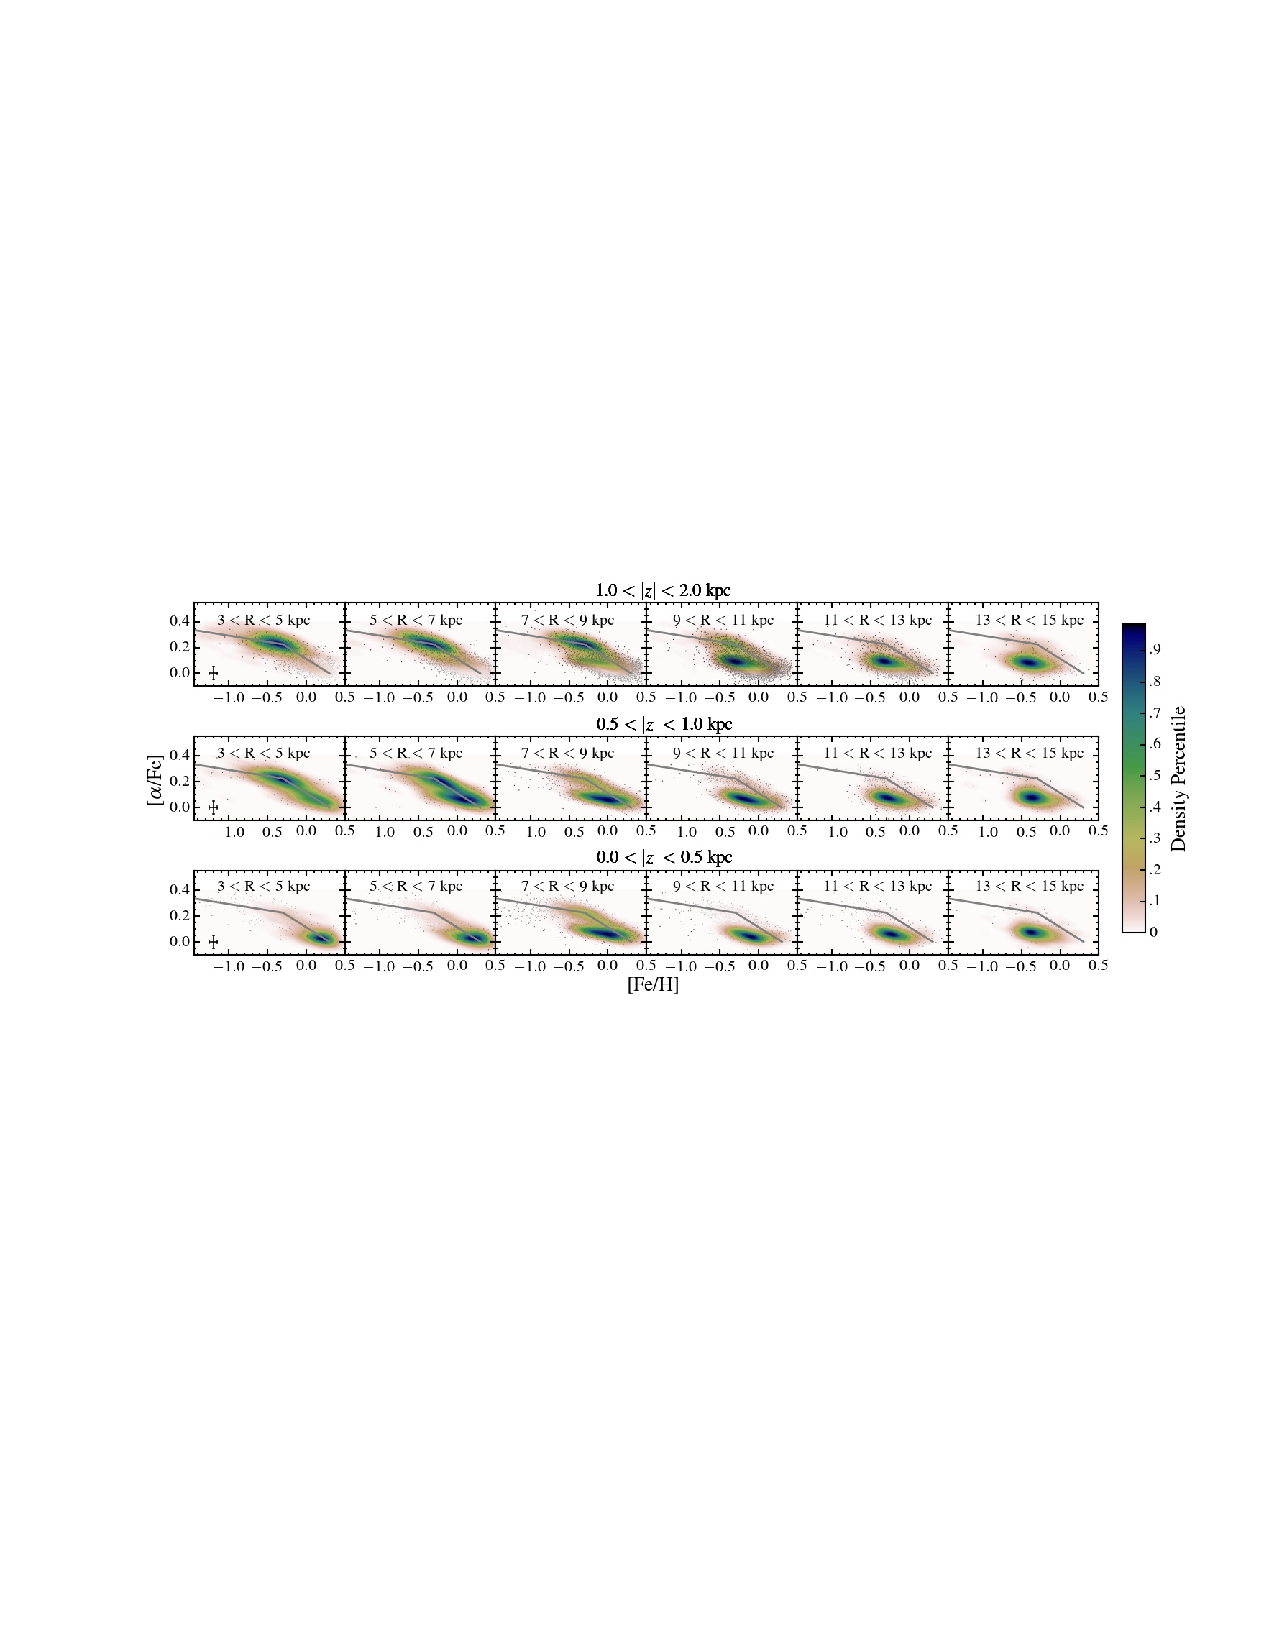
\includegraphics[width=\textwidth]{Introduction/figs/hayden_15.pdf}
  \caption[Metallicity and abundance of solar cylinder stars as a
  function of radius and
  height]{\fixspacing\label{intro:fig:hayden}The distribution of stars
    near the Sun in the [$\alpha$/Fe] vs. [Fe/H] plane, presented in a
    grid of radius and height. From \citet{Hayden15}.}
\end{figure}

By the middle of the last century it was well established that the
scale-heights and velocity dispersions of stars in the solar
neighborhood increase with age \citep[see][for a summary of this early
work, particularly the chapters contributed by Elvius and
Delhaye]{Blaauw65}. The seminal work by \citet{Roman50} demonstrated
that the disk kinematics also depended on metallicity.  Today these
patterns are known in the literature on Galactic archaeology as
age-velocity-metallicity (abundance) relations \citep[AVM$\alpha$-R;
e.g.,][]{Aumer09,Minchev14}. Observational advances continued for the
solar neighborhood \citep[e.g.,][]{Edvardsson93, Dehnen98,
  Nordstrom04}, and by the beginning of this century the complexity of
these relations had been mapped throughout much of Milky Way (MW) by
wide-field spectroscopic surveys (e.g., RAVE, \citealt{steinmetz06a};
BRAVA, \citealt{howard08a}, SEGUE, \citealt{yanny09a}, LAMOST,
\citealt{zhao12a} GALAH, \citealt{desilva15a},
Gaia-ESO,\citealt{gilmore12a}; and APOGEE-1 and -2,
\citealt{Majewski15}). The radial gradients in these relations are
beautifully shown in Figure \ref{intro:fig:hayden} (from
\citet{Hayden15}), illustrating the usefulness of both metallicity and
abundance as well-known, complementary chemical-evolutionary
tracers. Despite a century of remarkable progress, two broad but
intertwined questions remain: (i) What are the astrophysical processes
(i.e., the chemo-dynamical explanation) leading to the observed
relations?; and (ii) are these patterns generic for spiral disks or
specific to the Milky Way?

\begin{figure}
  \centering
  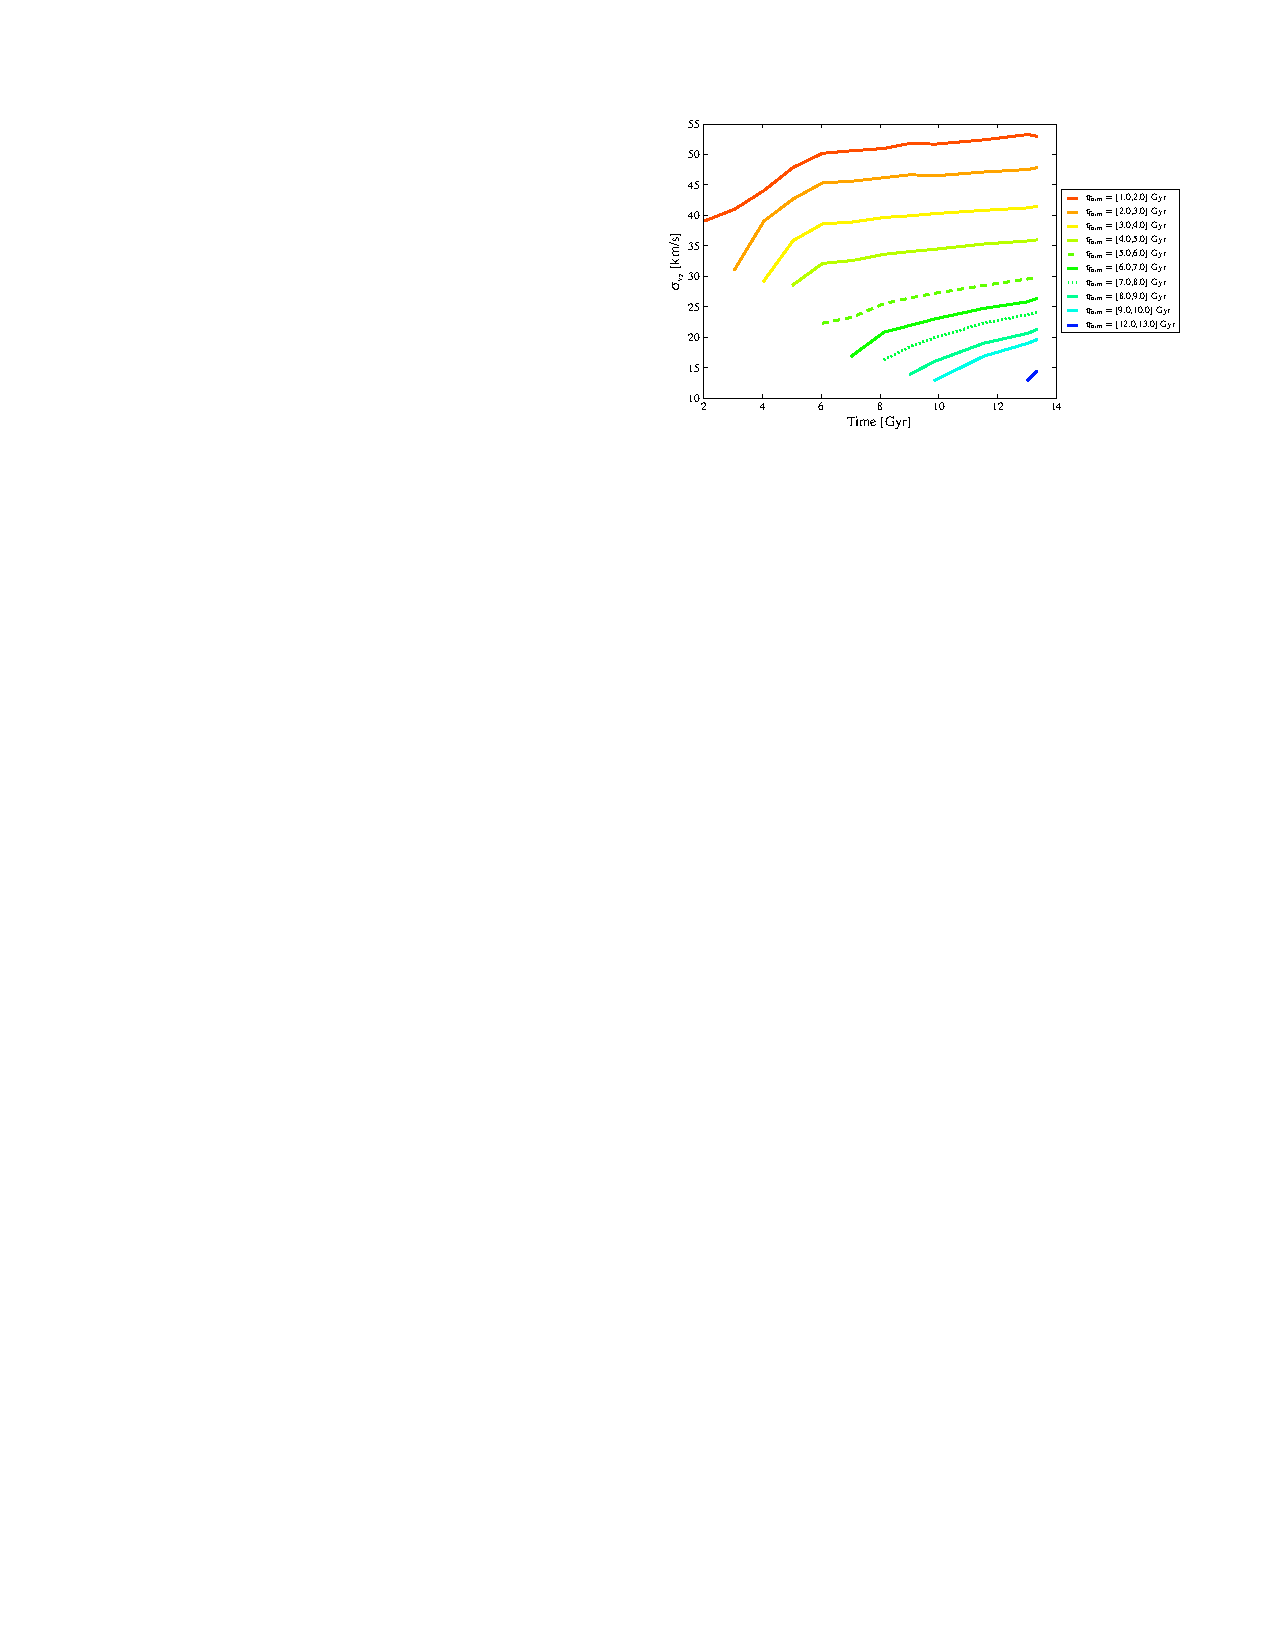
\includegraphics[width=0.8\textwidth]{Introduction/figs/bird_13.pdf}
  \caption[Dynamical settling in a Milky-Way-like galaxy
  model]{\fixspacing\label{intro:fig:bird}Vertical velocity dispersion
    of stellar populations with different formation ages as a function
    of time. These models are based on hydrodynamical simulations of a
    Milky-Way-like disk galaxy. From \citet{Bird13}}
\end{figure}

Setting aside chemical evolution for simplicity, there has been a
long-standing debate about the origin of the vertical stratification
of disk stars in phase-space as a function of age. This stratification
is known as the the age-velocity relation, or AV-R. Historically the
argument has been in the context of dynamical heating from two-body
scattering \citep{Spitzer51}, but the source of this scattering has
been debated \citep[e.g., giant molecular clouds, transient spiral
structure, or dwarf satellite
galaxies][]{Spitzer51,Spitzer53,Wielen77,Quinn93,Binney00}, and none
have proven satisfactory to explain the MW's thick disk.  This
framework has been salvaged but also up-ended by relatively recent
evidence for the increasing turbulence (and presumably thickness) of
ionized gas in disks at higher redshifts
\citep{Weiner06,Forster-Schreiber09,Wisnioski15}. It seems plausible
that early phases of disk formation involved gas cooling, leaving
behind an old, thick-disk stellar component
\citep{Brook04,Bournaud09}. However, thinner relic layers would also
emerge as time progressed \citep{Bird13}, depending critically on the
cooling time-scale for the gas in the presence of star-formation, AGN
feedback, and accretion. Figure \ref{intro:fig:bird} shows an example
of this theory; vertical velocity dispersion does slightly increase as
stars age (i.e. ``heating''), but the dominant trend is that more
recently formed populations are dynamically cooler. Ironically, this
``settling'' of the stellar disk is not unlike the predictions of
monolithic collapse from \citet{ELS}, albeit now consistent in the
context of bottom-up, or hierarchical structure formation as seen in
recent simulations \citep[e.g.,][]{Bird13,Martig14a}.  It is no longer
clear if, loosely speaking, disks ``heat'' or ``cool'' to form the the
vertical stratification of disk stars in phase-space, and likely both
modes play a role at late and early times, respectively. For this
reason we refer instead to ``dynamical stratification'' as a
phenomenon that captures both general physical processes.

The recent simulations noted above show there is a rich history of
radial and vertical build up of stellar populations that involves an
interplay between the cooling of the gas, the impact of mergers and
accretion, and, at late times, the classical heating processes noted
above.  This richness suggests the possibility for a diversity of
astrophysical paths in disk formation that could lead to significantly
different structure in galaxies, exhibited in their
AVM$\alpha$-Rs. Hence, the broader question of whether the MW is
representative of the external disk galaxy population becomes salient.

%% Maybe move to previous section
Little is known about the dynamical stratification rates for stars in
spiral galaxies outside the Milky Way, but recent studies of stellar
populations and dynamical stratification in low-mass spiral galaxies
\citep{Seth05a,Bernard15} have shown dramatic differences in the
age-metallicty and age-velocity dispersion relations when compared to
the Milky Way. Recent measurements of the stellar velocity dispersions
in M31 \citep{Dorman15} show that there are gradients in dispersion
with age and metallicity, but with amplitudes and time-scales that are
larger than in the MW. Differences in velocity dispersion amplitudes
may reflect a more massive or thinner M31 disk, but possibly also a
different dynamical history -- for gas settling or stellar dynamical
heating. Clearly more data on the stellar properties of external
galaxies is needed. The above studies serve as a gold standard since
they are based on studies of resolved stellar populations. Because
there are no massive spiral galaxies outside of the Local Group for
which we can resolve stellar populations at surface-densities high
enough to probe most of the disk, it is imperative to undertake
studies based on integrated starlight.

\section{Deriving Population Properties with Full Spectrum Fitting}
\label{intro:sec:SSP}
\begin{figure}
  \centering
  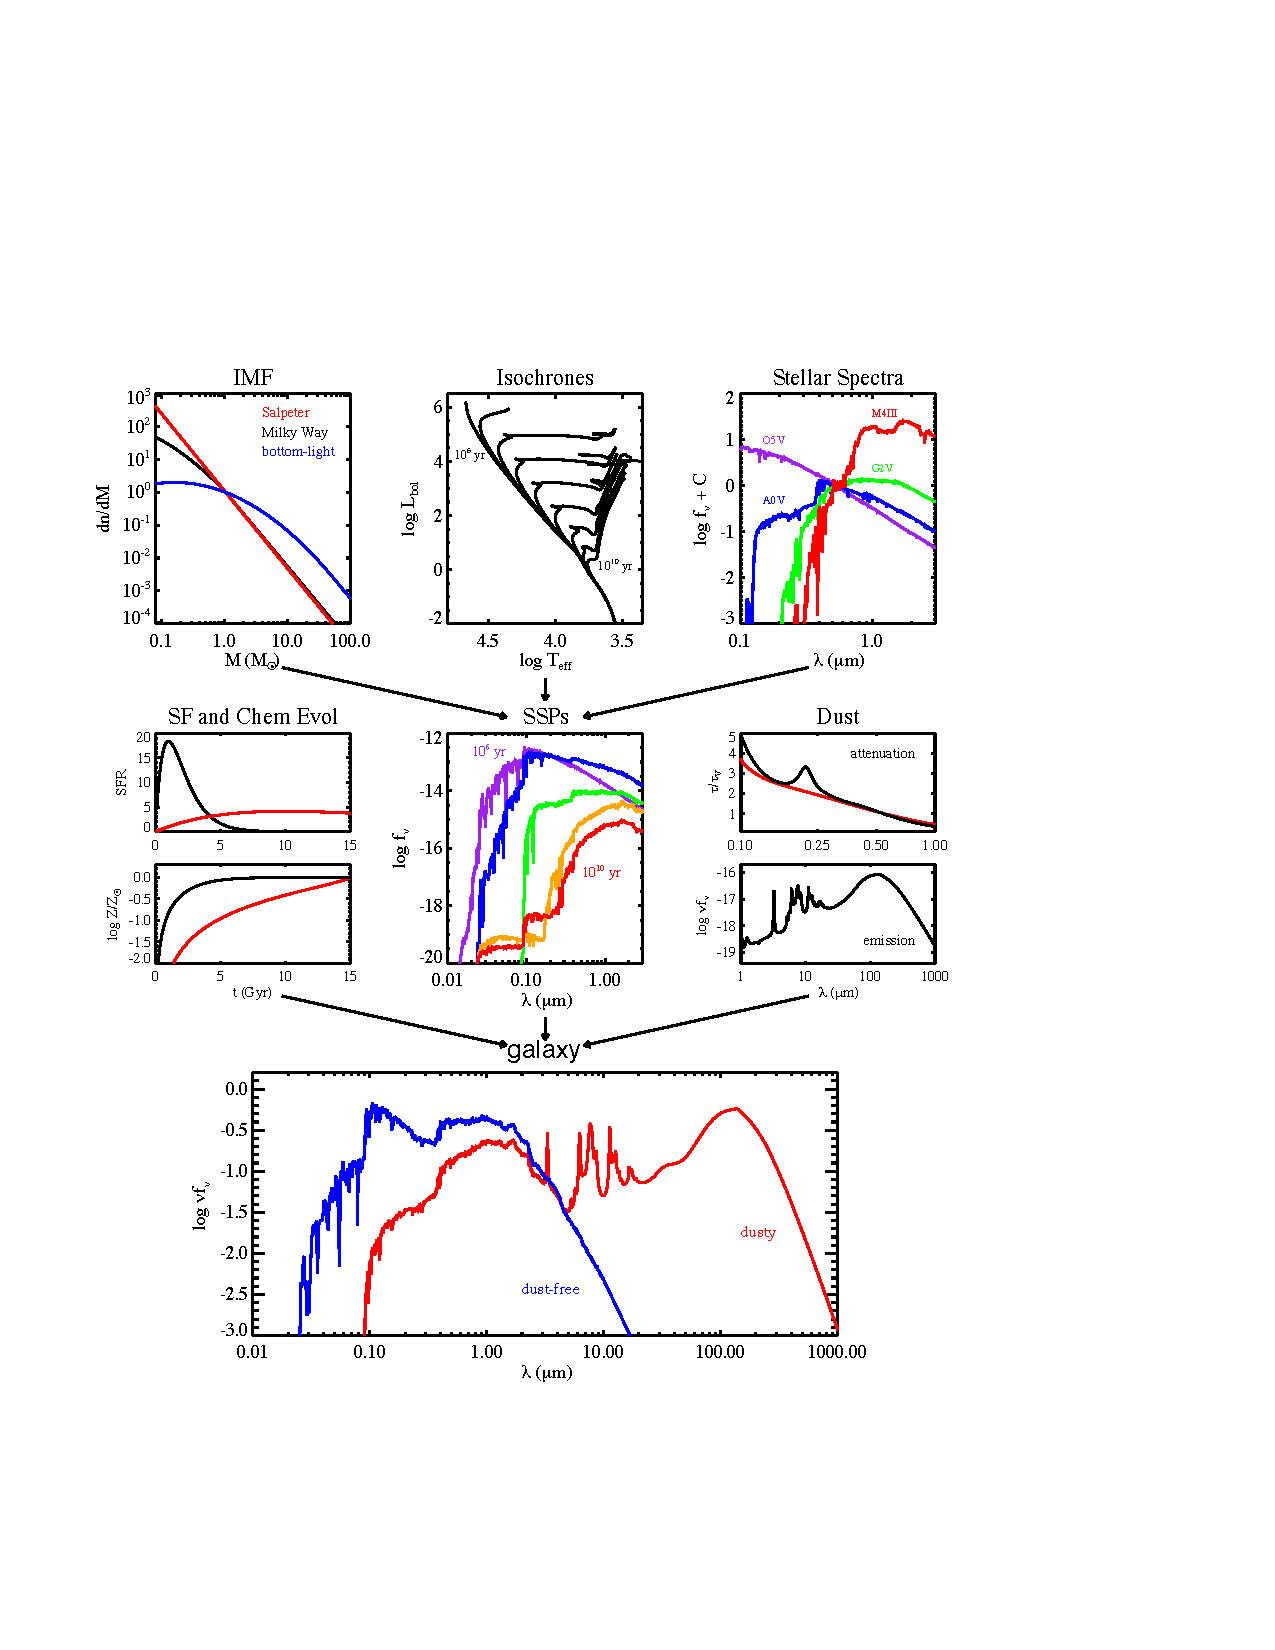
\includegraphics[width=0.8\textwidth]{Introduction/figs/conroy_13.pdf}
  \caption[Schematic of full spectrum
  fitting]{\fixspacing\label{intro:fig:conroy}The important components
    of full spectrum fitting. An initial mass function (IMF),
    isochrones, and spectra are combined to construct individual
    SSPs. Multiple SSPs are then combined, with and assumed star
    formation history and dust properties, to form a model
    galaxy. From \citet{Conroy13}.}
\end{figure}

In this work we employ full-spectral fitting to measure age,
metallicity, and extinction as a function of radius and height in NGC
891. The idea of modeling integrated starlight (i.e., a spectrum) to
measure galaxies properties has a long history since \citet{Spinrad71}
first manually mixed stars together, and modern techniques employ a
variety of sophisticated methods to extract the maximum about of data
from each wavelength. Regardless of the specific method, all attempts
at full-spectrum fitting require the same basic ingredients: (i) a
library of stellar spectra, whether empirical or synthetic, (ii) a set
of isochrones that encapsulate how stars evolve with time, and (iii)
an initial mass function (IMF). With these three components
Astronomers can construct simple stellar populations (SSPs); a set of
stars of the same age and same metallicity/abundance with a mass
distribution determined by the IMF. To simulate an entire galaxy
multiple SSPs of different ages and metallicities are combine together
to produce a complex stellar population (CSP), which requires assuming
both a star formation history (SFH) and the distribution/properties of
dust in the galaxy. An excellent discussion of this process can be
found in \citet[and his diagram shown in Figure
  \ref{intro:fig:conroy}]{Conroy13}.

Within the general picture painted above there exists a wide range of
options and data. It is common for SSP libraries to be constructed
with the Padova isochrones \citep{Bertelli94, Girardi00, Marigo08}
because these models cover the widest range of stellar age and
chemical compositions, but other models are often used for their focus
on specific epochs of stellar evolution. For example high-mass stars
(Geneva \citep{Schaller92,Meynet00}), low-mass stars ($Y^2$
\citep{Yi01,Yi03}, or Dartmouth \citep{Dotter08}), and even very
low-mass stars (Lyon \citep{Chabrier97,Baraffe98}). In this work we
use exclusively the Padova isochrones because our observations, by
their very nature, are light-weighted and therefore the specific
details of low mass stars are relatively unimportant.

The choice of IMF can also affect the final modeled galaxy
spectrum. The canonical IMF of \citet{Salpeter55} was based on
observations of the Solar Cylinder in the Milky Way, and there is so
far little evidence that the IMF is appreciably different elsewhere in
the Universe \citep{Bastian10}. More recent observations have refined
the specific form of the IMF \citep{Kroupa01, Chabrier03}, but the
general picture remains the same. We use the IMF of \citet{Chabrier03}
because it is physically motivated and provides a good fit to low-mass
and brown dwarf star counts in the Milky Way
\citep{Bruzual03,Chabrier01,Chabrier03}.

Finally, the construction of SSPs depends on the stellar library
used. In this work we consider only empirical stellar libraries, and
more specifically the STELIB \citep{LeBorgne03} and MILES
\citep{Sanchez-Blazquez06} libraries. The main strength of empirical
libraries is that they get the chemistry right by default, as indeed
they must. The cost of this accuracy, however, is a very limit
sampling of the entire parameter space of stellar evolution. For
example, as is discussed in \S\ref{891_2:sec:ma11}, the MILES library
very coarsely samples the metallicty/age plane and doesn't have any
spectra for ages below \val{6.5}{Myr}. 
% Ultimately, we use the STELIB
% library because it more finely samples stars of different ages, but
% warn that it still lacks a detailed view of how spectra change with
% metallicity.
As discussed in \S\ref{891_2:sec:SSP_sets} we ultimately use the SSPs
of \citet{Bruzual03}, which are constructed with the Padova
isochrones, Chabrier IMF, and STELIB library. We note, however, that
over the wavelength range we consider ($\val{3800}{\AA}
\leq\lambda\leq \val{6800}{\AA}$) the differences in spectral shape
caused by different assumptions/models are minimal.

More directly relevant to our work is the assumption about the SFH
that is used to construct galaxies (CSPs) from SSPs. A common choice
for SFH is the so called $\tau$-model where the star formation rate
(SFR) follows an exponential function with a single scale parameter,
$\tau_\mathrm{SF}$. This analytic form is based on closed-box models
where the SFR depends linearly on gas density \citep{Schmidt59} and
offers an attractive, one parameter, parameterization of the SFH. In
this work we chose to use a non-parametric SFH (as discussed in
\S\ref{891_2:sec:SSP_method}) which allows us to reduce the
systematics in our results that arise from forcing an analytic form of
the SFR (systematics are not completely eliminated, however, as
discussed in \S\ref{891_2:sec:sys_err}). Using this method results in
a much larger set of free parameters and puts more strain on the
fitting code, but our data have high enough signal to noise
(\val{\asim 30}{px^{-1}}) to make it a viable option.

Once model galaxies are constructed there are a multitude of methods
available to fit them to our data, for example those of
\citep{Cappellari04, Tojeiro07,Chen12, CidFernandes05, Ocvirk06,
  Wilkinson15, Sanchez16}. Regardless of the method used these fits
face the same common issues; namely how to deal with known
degeneracies between age, metallicity, and extinction
\citep{Oconnel76,Aaronson78,Worthey94,dePaz02}. In some methods the
extinction degeneracy can be mitigated by removing the overall
continuum from both the data and models before fitting
\citep[e.g.,][]{Ocvirk06,Wilkinson15} and then recovering an
extinction estimate either by measurements of gas emission (i.e., the
Balmer decrement) or separate analysis of the ``best fit'' galaxy
spectrum. Metallicity and age are more closely entwined and the
degeneracy between them more difficult to break. In this work we
attempt to quantify the uncertainties that arise from similarities
between SSPs that are degenerate with age and metallicity (see
\S\ref{sec:fit_err}), but note that we have not addressed systematic
uncertainties that may arise from our choice of model SSPs.

\section{A Fiber Optic Primer}
\label{intro:sec:fiber}
The use of fused silica optical fibers for astronomical observations
was first suggest by \citet{Angel77}, and in the intervening decades
their importance and usefulness to Astronomy has only increased. The
astronomical benefits of fiber optics are essentially two fold:
Firstly, they allow instruments to be decoupled from the telescope
focal plane, which enables the construction of very large and
sensitive spectrographs that are free from the unstable environmental
conditions often found on the observing floor. Secondly, they can be
easily placed at an arbitrary position on the sky while maintaining a
consistent spectrograph input.

A class of fiber optic instruments called integral field units (IFUs)
make great use of this second point. IFUs are a collection of fibers
that are placed in some two-dimensional configuration on the sky and
therefore produce data that exist in three dimensions (two spatial and
one spectral). Some IFUs are designed to efficiently measure the
spectra of a large field of stars, for example HYDRA {\bf REF? Can't
  find it!}, and can have the location of their fibers changed from
program to program. Others have a fiber layout that is fixed and
usually intended for observations of extended objects. SparsePak
\citep{Bershady04,Bershady05} is an excellent example of and IFU of
this type. The trade off for the lack of reconfigurability in fixed
IFUs is a generally tighter fiber packing and therefore improved
spatial coverage.

In the past, difficulties in construction resulted in a cottage
industry of IFU builders, but more recently there has been an
explosion of mass-produced IFUs that have allowed large, resolved
spectrographic surveys like MaNGA \citep{Bundy15}, SAMI
\citep{Croom12}, and CALIFA \citep{Sanchez12} to rapidly expand our
view of the Universe. In this thesis I present \GP and HexPak, a set
of IFUs that are the first in the world to contain fibers of different
sizes, each configured to serve a specific scientific purpose.

\begin{figure}
  \centering
  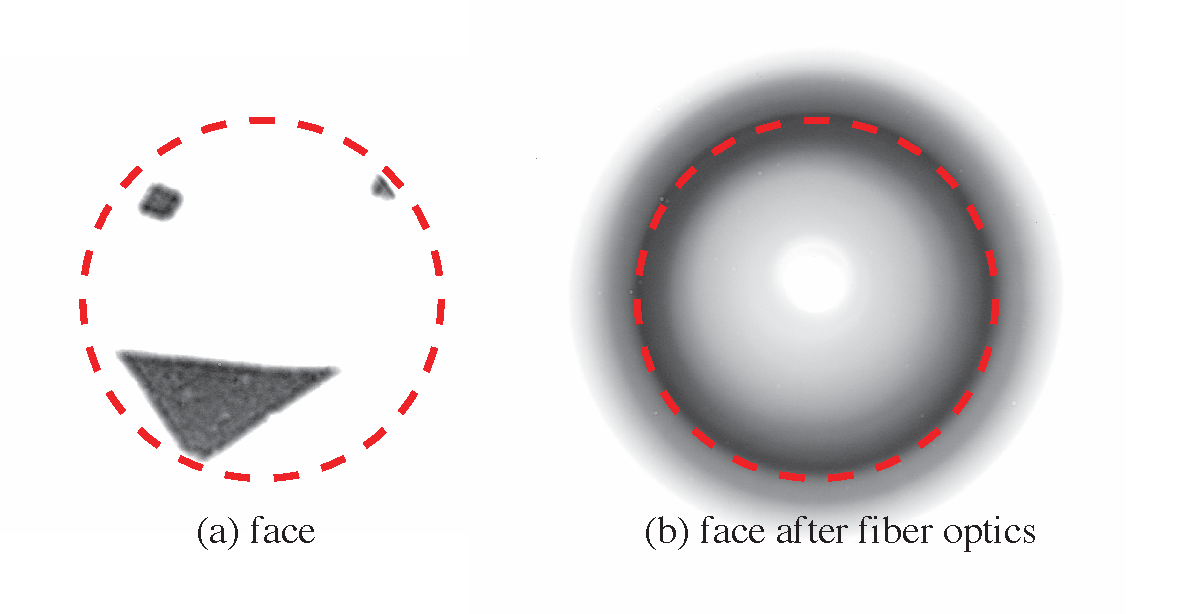
\includegraphics[width=\textwidth]{Introduction/figs/FRDude.pdf}
  \caption[Face on FRD]{\fixspacing\label{intro:fig:FRDude}The effects
    of fiber optics on an input signal. The face in (a) is smeared
    azimuthally and radially during its journey through an optical
    fiber. The red circle corresponds to the same angle at the
    input/output of the fiber.}
\end{figure}

With great power comes great responsibility, however, and fiber optics
affect the light passing through them in ways that have profound
implications for data quality and instrument design. In particular,
fiber optics not only attenuate precious astronomical light, but also
increase the entropy in the beam. The latter effect is referred to as
focal ratio degradation (FRD), whereby light injected into a fiber at
a particular angle emerges from the fiber at a larger angle. An
example of this is seen in Figure \ref{intro:fig:FRDude}; the light
coming out of the fiber (b) has been smeared to angles outside of the
maximum input angle (red circle). This increase in entropy creates a
need for larger (and more expensive) spectrograph optics and can
decrease the total system throughput if not properly accounted for. An
understanding of the causes of FRD can help mitigate its effects and
the first theories placed the blame on microbends along the length of
the fiber \citep{Gloge72,Carrasco94}. Recent studies have suggested
however, that most FRD is caused by scattering at the surface of the
fiber \citep{Avila98,Haynes11,Eigenbrot12}. In the latter scenario it
is likely that surface treatments (i.e., anti-reflective coatings) can
mitigate the effects of FRD.

\clearpage
\phantomsection % Fixes references link in hyperref/PDF index

% Requires thesis.bst to be present (or linked) in chapter subdirectory.
\bibliographystyle{thesis}
\bibliography{Introduction}

\chapter[Fiber Focal Ration Degradation]{The Angular and Wavelength Dependence of Fiber Focal Ratio Degradation}
\label{chap:FRD}
\epigraph{\fixspacing\emph{Every hidden cell is throbbing with music
    and life, every fiber thrilling like harp strings.}}{John Muir}
% Leave space between title and quote or publication note.  This has often been
% 10cm for a quote and 8 cm for a reference, but this is really up to you.
%\vspace{8cm}
\vfill

\begin{flushright}
  \fixspacing
  \textit{A version of this chapter has previously appeared in\\
    \emph{Ground-based and Airborne Instrumentation for Astronomy IV. Proceedings of the SPIE}}\\
    \vspace{1ex}
    Eigenbrot, Bershady, and Wood 2012. Volume 8446 article 84465W
\end{flushright}

\vspace{1in}

\cleardoublepage

%%%%%%%%%%%%%%%%%%%%%%%%%%%%%%%%%%%%%%%%%%%%%%%%%%%%%%%%%%%%% 
\begin{chabstract}
  We present measurements of how multimode fiber focal-ratio degradation
  (FRD) and throughput vary with levels of fiber surface polish from 60
  to 0.5 micron grit. Measurements used full-beam and laser injection
  methods at wavelengths between 0.4 and 0.8 microns on 17 meter lengths
  of Polymicro FBP 300 and 400\mum\ core fiber. Full-beam injection
  probed input focal-ratios between \f3 and \f13.5, while laser
  injection allowed us to isolate FRD at discrete injection angles up to
  17 degrees (\f1.6 marginal ray). We find (1) FRD effects decrease as
  grit size decreases, with the largest gains in beam quality occurring
  at grit sizes above 5\mum; (2) total throughput increases as grit
  size decreases, reaching 90\% at \filtI with the finest polishing
  levels; (3) total throughput is higher at redder wavelengths for
  coarser polishing grit, indicating surface-scattering as the primary
  source of loss. We also quantify the angular dependence of FRD as a
  function of polishing level. Our results indicate that a commonly
  adopted micro-bending model for FRD is a poor descriptor of the
  observed phenomenon.
\end{chabstract}
\cleardoublepage

\section{Introduction}

Multimode optical fibers provide the most cost-effective coupling
between telescopes and spectrographs that allow spectrographs to be
placed in stable environments. However, these fiber optics contribute
to light loss from attenuation within the fiber material and
surface-scattering of their ends, and increase entropy in the optical
beam. The latter effect is referred to as focal ratio degradation
(FRD), whereby light injected into a fiber at a particular \fratio
emerges at a faster (smaller) \fratio. Ever since the first efforts to
characterize FRD in astronomical applications \citep{Angel77}
astronomers have attempted to understand its cause(s) in the hope to
lessen its effects \citep{Carrasco,Oliveira}. Microbends have
historically been a favored culprit \citep{Carrasco,Gloge72}, but
recently it has been suggested \citep{Haynes11, Avila98} that scattering
caused by surface-roughness on the fiber face contributes
significantly to FRD.

We discuss the results of two experiments designed to measure how the
amount of FRD depends on surface roughness, wavelength, and input
angle. The experiments described here use both full-beam and laser
injection methods \citep{Carrasco} standard for FRD tests in
astronomical applications. The full-beam method is useful for
characterizing how a fiber would perform when fed by a telescope,
and provides a straightforward way to compute practical metrics useful
for designing spectroscopic instruments. The laser injection method
allows light to be injected into the fiber at discrete input angles
(compared to a filled ray-bundle cone). This angular dependence of
scattering is a particularly sensitive diagnostic of the physical
mechanisms responsible for FRD.

The method and results of our experiment of FRD dependence on surface
roughness are presented in \S \ref{FRD:sec:polish}. Results for the
wavelength dependence of FRD are reported in \S
\ref{FRD:sec:wavelength}. The dependence of scattering on input angle is
reported in \S \ref{FRD:sec:angle}, and the implications of our work are
discussed in \S \ref{FRD:sec:summary}.

\section{Grit Size and Wavelength Dependence}
\label{FRD:sec:polish}
\subsection{Polishing Method}
\begin{figure}[ht]
    \includegraphics[width=1.0\textwidth]{FRD/figs/mosaic.eps}
    \caption[Fiber face with varying degrees of polish]{\fixspacing Images of
      the ``test'' surface of the fiber cable showing the appearance of the
      fiber face at each of the six stages of polishing. The number in the
      bottom right corner of each panel denotes the size of grit used. The
      fiber core diameter is 300$\mu$m.\label{fig:mosaic}}
\end{figure}

Our tests used Polymicro Technologies stepped-index broadband optical
fibers, cut to $\sim$17 meters in length.  FBP300330370 has
core:clad:buffer diameters of 300:330:370\mum, respectively; a second
length of FBP400440480 has 400:440:480\mum\ diameters.  We mounted
each fiber end into 0.25 inch cylindrical brass ferrules using Norland
Optical Adhesive 61 ultraviolet-curing epoxy.

The experiment was designed to maintain one end of each fiber cable as
a ``control'' surface, well-polished (0.5\mum) at the beginning of
testing, and to use the other end of the fiber cable as the ``test''
surface, initially polished using a coarse grit and then re-polished
with successively finer grit sizes after each measurement.  For
creating the progression of decreasing surface roughness we performed
consecutive polishing steps on the test surface using silicon carbide
lapping disks of 60, 30, 15, 5, and 1\mum\ grit as well as 0.5
\mum\ grit aluminum oxide disks.

The fiber cable was polished using an Ultra Tec Manufacturing, Inc.,
ULTRAPOL 1200-series lapping machine.  We considered a fiber surface
to be adequately polished when, under visual inspection, surface
grooves appeared to be relatively even across the face with very few
surface features larger than the grit size used to polish the surface.
We imaged each end of the fiber using a Newport Corporation F-ML1
fiber inspection microscope for magnification and a Motic Corporation
Moticam 2300 CMOS detector.  We took images after each polishing step
in order to confirm that the test surface was adequately polished and
that the control surface remained undamaged.  We also captured images
after each FRD measurement step in order to determine if the fiber
faces had been damaged during handling, as any potential damage could
affect the test results.  A mosaic of images of the test surface, as
seen after the FRD measurement at each grit size, is seen in
Figure~\ref{fig:mosaic}.


\subsection{Data Collection}
\label{FRD:sec:direct}
The experimental apparatus is a modified version of the far-field
differential beam comparator using a double re-imaging system
described in \citet{Crause_08}, which is based of the FRD test
apparatus used to characterize the fibers of SPARSPAK
\citep{Mab_04}. The final collimating lens (L3 in \citet{Crause_08})
was replaced with a Canon \f1.2 camera lens to eliminate ghost images
caused by very fast output beams. Stray light was further reduced by
covering everything downstream of the focus plane with a black
photographer's cloth. The fiber input stage was replaced with a highly
stable, purpose-built three-axis translation stage that ensures the
fiber face is telecentric to within $0.01^{\circ}$. Finally, a filter
magazine was added to the pinhole assembly to facilitate the rapid
changing of filters.

Basic operation involves recording data from two imaging modes; the
far-field fiber output, and the far-field image of the direct
beam. The level of FRD is then computed by comparing the two modes.
Examples of these images are shown in Figure \ref{fig:dfim},
illustrating the increasing impact of FRD at slower beam-speeds. Data
were taken in three filters: Johnson I and B and Stromgren \emph{y},
with central wavelengths of \filtI, \filtB, \filty, and widths of
$\Delta\lambda/\lambda=$ 0.22, 0.19, 0.045, respectively; four
$f$-ratios (\f3, \f4.2, \f6.3, and \f13.5); and five polish
levels (60, 30, 15, 5, and 1\mum). The range in $f$-ratios was chosen
so that results are applicable to a wide range of telescope
designs. The Wisconsin Indiana Yale NOAO (WIYN) 3.5m telescope has a
\f6.3 Nasmyth port; the Sloan Digital Sky Survey Telescope fibers
are fed at \f5; and the South African Large Telescope (SALT) feeds its
prime focus instrument package at \f4.2 (similar to the Hobby Eberly
Telescope).

Throughput measurements require very precise knowledge of the
intrinsic lamp output (the light input to the system). Experiments in
lab showed that, while the stochastic variations of the lamp are
negligible, there is a secular drift towards lower lamp
output. Subsequent to the experiment reported here a photo-diode
monitoring system has been implemented to correct for this trend. The
data presented here accounted for this trend by: 1) taking a set of
images for one filter with the fiber in place, 2) taking a set of
direct beam images in the same filter, 3) repeating this alternating
scheme until three groups of fiber images, separated by two groups of
direct beam images were taken. This alternating fiber-direct-fiber
scheme is used to remove stochastic lamp variability.

Images were cleaned of detector artifacts and combined to produce five
images for each filter at each polish level: three fiber images and
two direct beam images. Lamp variations were removed by using the
three fiber images as data points to determine a lamp normalization
(relative to the first fiber image) as a function of time. This
function was then used to find normalizations for the direct beam
images. The lamp was found to have no significant variation (10\% of the shot noise)
 within the time required to take one set of data in a particular filter.

\begin{figure}[ht]
\centering

\includegraphics[width=0.25\textwidth]{FRD/figs/bdirect_3.eps}
\includegraphics[width=0.25\textwidth]{FRD/figs/bdirect_42.eps}
\includegraphics[width=0.25\textwidth]{FRD/figs/bdirect_63.eps}
\includegraphics[width=0.25\textwidth]{FRD/figs/bdirect_135.eps}\\

\includegraphics[width=0.25\textwidth]{FRD/figs/bfiber_3.eps}
\includegraphics[width=0.25\textwidth]{FRD/figs/bfiber_42.eps}
\includegraphics[width=0.25\textwidth]{FRD/figs/bfiber_63.eps}
\includegraphics[width=0.25\textwidth]{FRD/figs/bfiber_135.eps}
\caption[Input and output far-field
  images]{\fixspacing\label{fig:dfim}Far-field images of the direct-beam (top)
  and fiber-beam (bottom) outputs for all $f$-ratios tested. Data shown is at
  \filty for the FBP300330370 fiber, 17m in length. Direct and fiber beam
  images for a given \fratio have identical spatial scales, and are adjusted
  such that the direct beam images are the same apparent size for all
  $f$-ratios.}
\end{figure}

\subsection{Analysis}
A custom data reduction pipeline was created to consistently and
efficiently analyze the large volume of data associated with the
multiple filters and polish levels. Analysis consisted of measuring
the total light contained within annuli of constant width and
increasing radius centered on the center of the beam. This information
was then used to construct a curve of growth that shows the fractional
encircled energy (EE) as a function of radius.

In addition to FRD, there are aberrations inherent in our test
apparatus that will affect both the direct beam and fiber beam in the
same way. To remove the effects of these aberrations the difference
between the direct beam and a theoretical ideal beam (no aberrations)
is computed and applied to both the fiber and direct beams;
\citet{Crause_08} provide a complete description of the method
used. Once the corrections have been applied the only differences
between the fiber and direct beams are caused by FRD.

\subsection{Results}
\label{FRD:sec:results}

\begin{figure}[ht]
\begin{center}
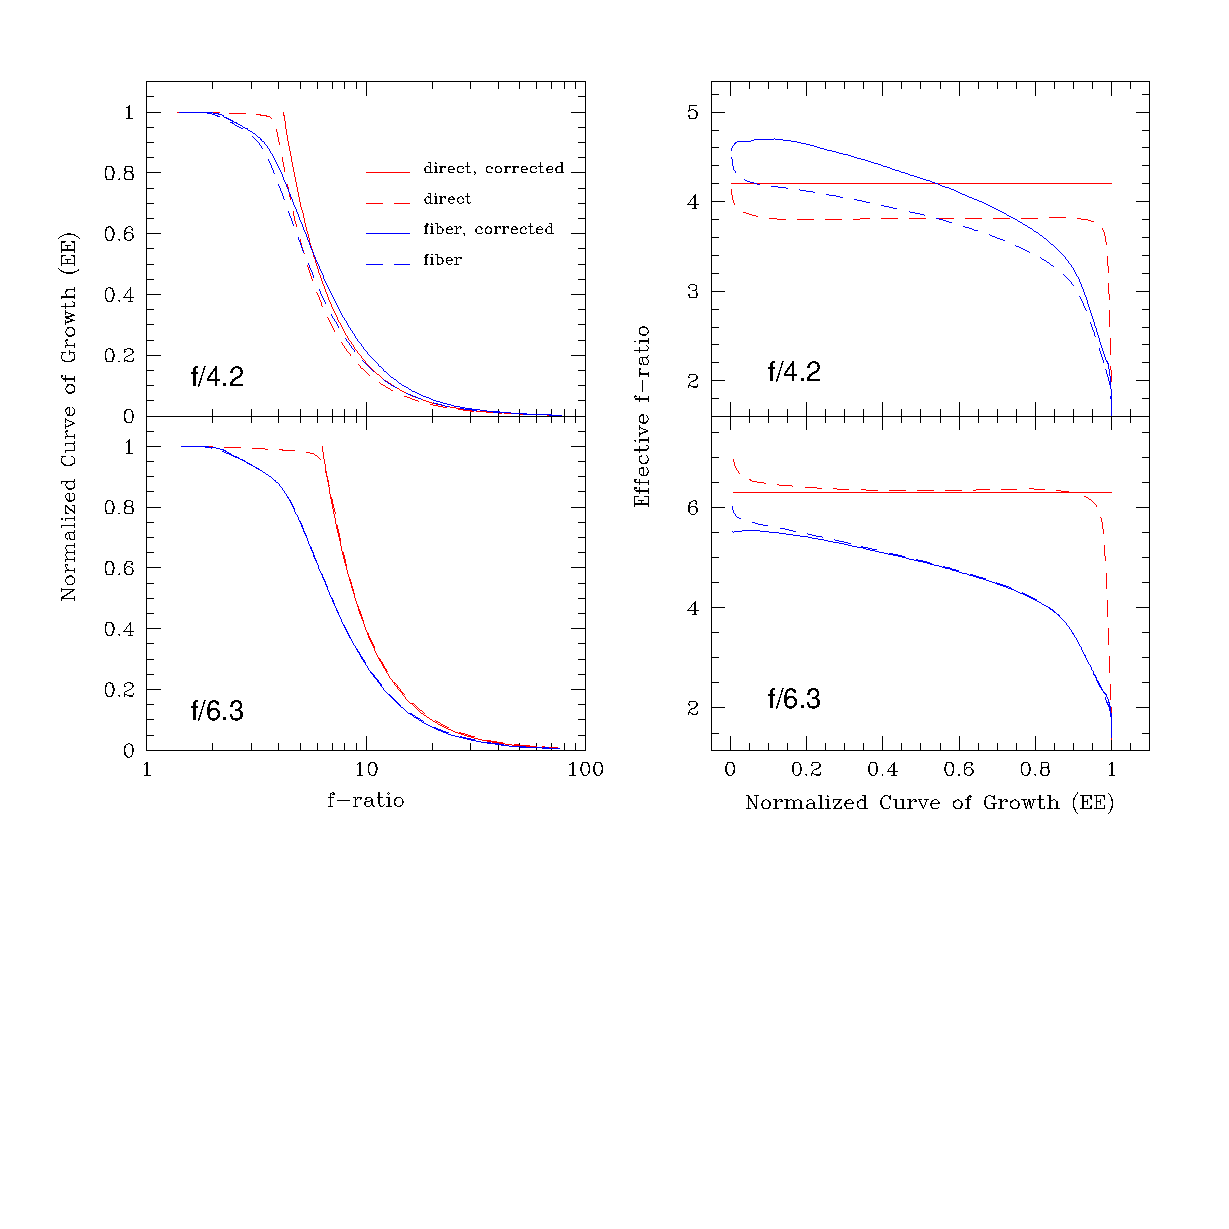
\includegraphics[width=\textwidth, trim=0 2.6in 0 0, clip=true]{FRD/figs/basic_FRD.eps}
\caption[Example FRD analysis plots]{\fixspacing\label{fig:basicFRD} FRD
  effects at \filty, \f4.2 and \f6.3, and with the output face polished to
  30\mum. The left panels show enclosed energy (EE) as a function of
  \fratio. The right panels show the effective \fratio of a beam that captures
  a certain percentage of the total light (EE). Data is for the FBP300330370
  fiber, 17m in length.}
\end{center}
\end{figure}

Figure \ref{fig:basicFRD} shows a characteristic set of FRD analysis
plots at a 30\mum\ end-polish at \f4.2 and \f6.3.  (See Figure
\ref{fig:grit} for more grit-sizes and \S\ref{FRD:sec:gritwave} for
discussion).  The left panels, which consist of normalized curves of
growth (COG) for both the direct and fiber beams, show how FRD
scatters light out to larger radii. The dashed and solid lines are the
data before and after the correction described above \citep{Crause_08}.

The right panels plot the effective \fratio as a function of
EE. These plots only show information about relative light
(re)distribution; they do not contain any information about total
throughput.  Where the fiber curve intersects the ideal beam tells us
what percentage of the original beam's information is being captured
by a spectrograph with an \fratio equal to that of the optics feeding
the fibers. This plot can also be used to estimate how much faster a
spectrograph would have to be to capture more of the input beam. For
example, from figure \ref{fig:basicFRD} and for fibers polished to 30\mum, an \f4.2
spectrograph only captures about 53\% of the light fed into the fibers 
at \f4.2. If we wanted to capture 90\% of the input light the
spectrograph optics would need to be \f3.2.

\subsubsection{Grit-size and \fratio Dependence}
\label{FRD:sec:gritwave}
\begin{figure}[htp]
  \centering
  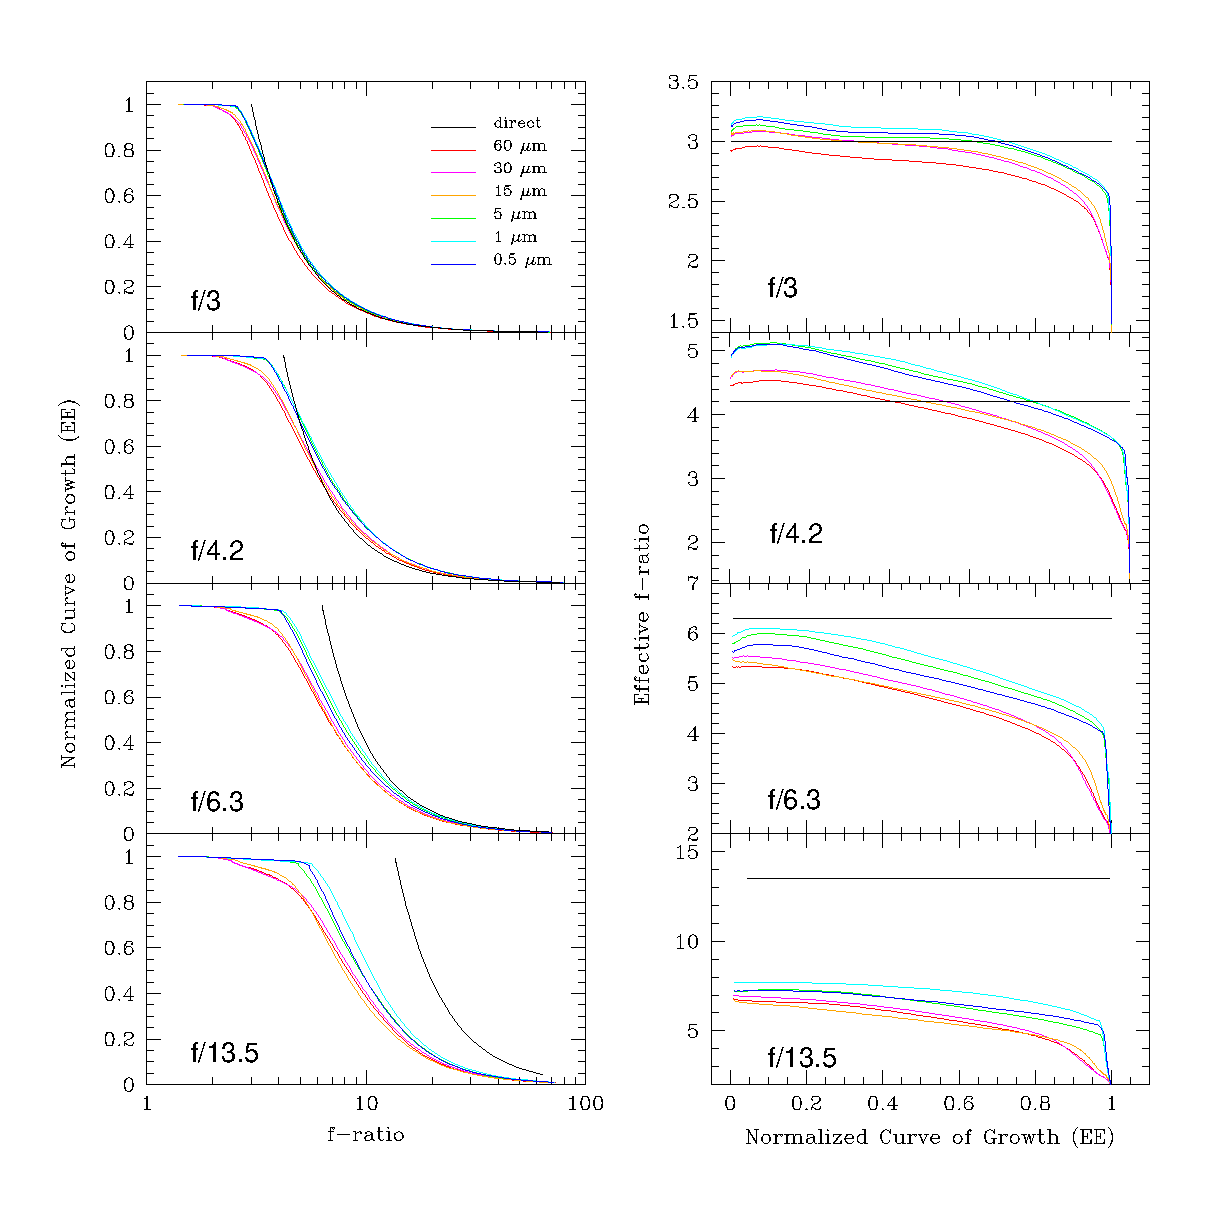
\includegraphics[width=\textwidth]{FRD/figs/gritplot.eps}
  \caption[Dependence of FRD on polish
    level]{\fixspacing\label{fig:grit}Dependence of FRD on polish grit size at
    \filty and all $f$-ratios measured for 17m of FBP300330370 fiber.}
\end{figure}

The primary result of the experiment can be seen in figure
\ref{fig:grit}, which shows FRD curves at one wavelength (\filty) and at
all of the different end-polish levels and $f$-ratios. As expected,
the effects of FRD improve as grit size decreases, but only to a
point. There is steady improvement in output beam quality between 60
\mum\ and 15\mum, a sharp improvement between 15\mum\ and 5\mum,
and almost no improvement between 5\mum\ and 0.5\mum.

It is also worth noting that for certain combinations of input \fratio
and polish level there is a radius (output \fratio) within which there
is relatively \emph{more} light in the fiber beam than in the direct
beam.  The explanation is straightforward: FRD scatters light from
each input angle into both larger and smaller output angles. If the
width of the scattering profile increases towards smaller angles (see
\S\ref{FRD:sec:angle}) then more light is scattered out of these angles
compared to larger angles. However, for a uniform input beam
larger input angles contain more luminosity (because they contain
larger annular areas) and so the amount of light scattered in from large
angles will exceed the amount of light scattered out from small angles
despite the wider scattering profile at small angles. In this case the
fiber beam will have relatively more light at smaller angles than the
direct beam, as seen in the plots for \f3 and \f4.2. Conversely,
there is some sufficiently large output angle that has
significant scattering contributions from angles where there is no
light in the input beam. At these output angles, the COG drops below
the ideal beam, as observed.

It is well known that FRD changes with changing input $f$-ratio,
increasing with slower beams \citet{Ramsey88}, as seen in Figure
\ref{fig:grit}.  For beams slower than \f6.3 the scattering becomes so
large that the output beam never contains more light than the input
beam for any angle.

\subsubsection{Wavelength Dependence and Total Throughput}
\label{FRD:sec:wavelength}
\begin{figure}[ht]
  \centering
  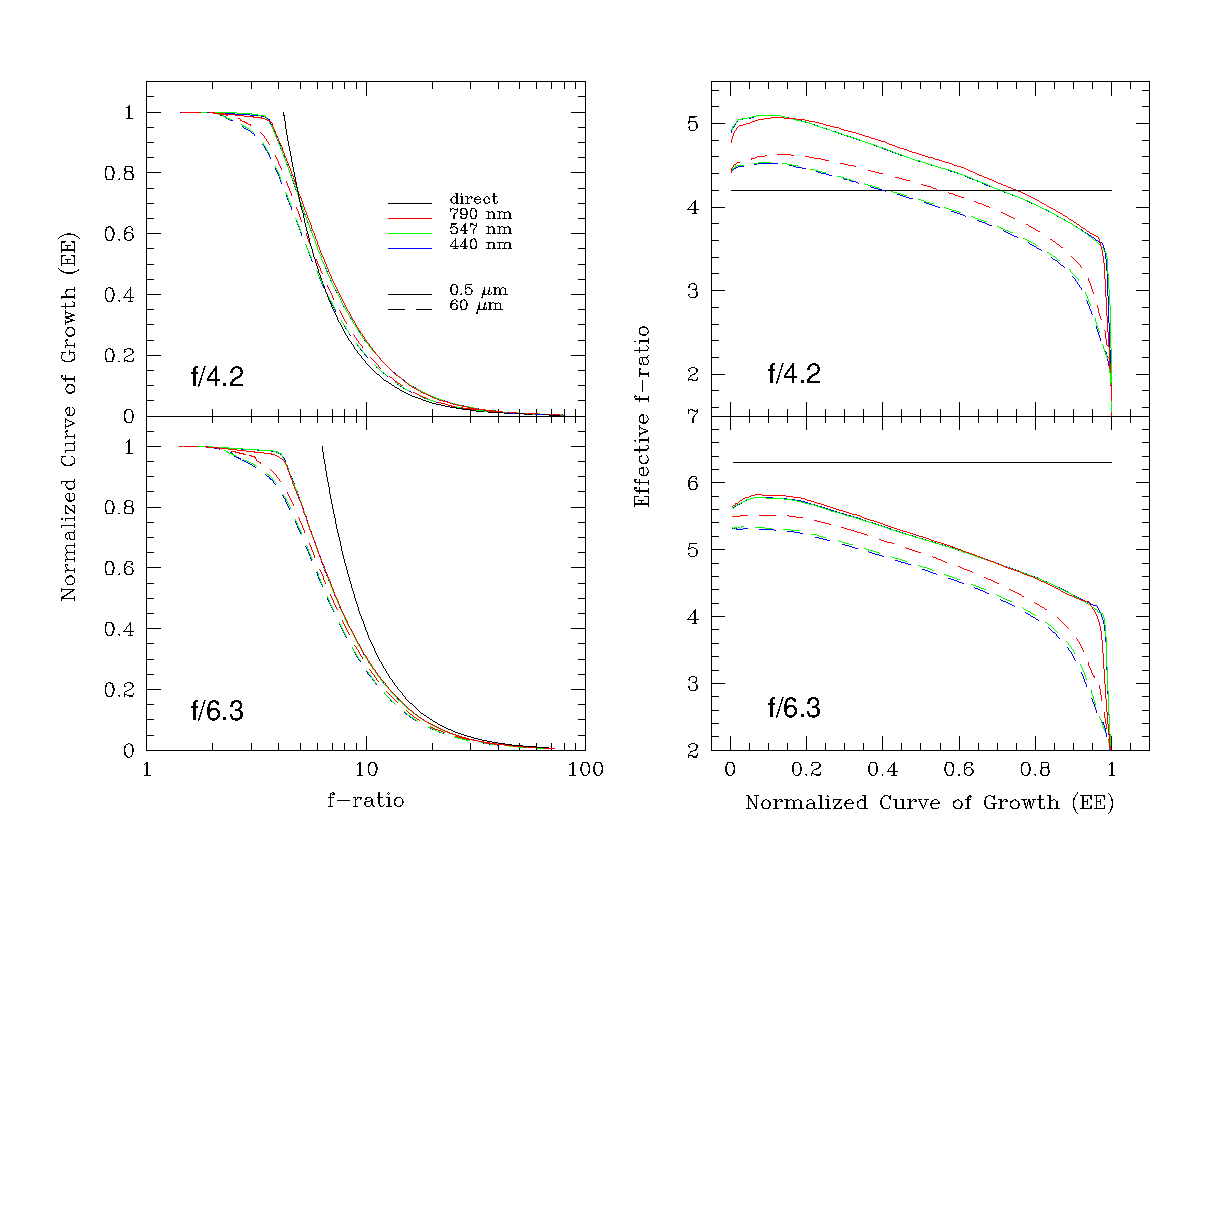
\includegraphics[width=\textwidth, trim=0 2.6in 0 0, clip=true]{FRD/figs/filters.eps}
  \caption[Dependence of FRD on wavelength]{\fixspacing\label{fig:wave}
    Wavelength dependence of FRD at 0.5 and 60 \mum\ polish grit at \f4.2
    and \f6.3 for 17m length FBP300330370 fiber.}
\end{figure}

Previous tests for a wavelength dependence on FRD have been split
between results that suggest there is such a
dependence \citep{Carrasco,Gloge72}, based on what would be predicted by
a micro-bend origin, and results that point to no wavelength
dependence \citep{Mab_04, Schmoll_03}. Figure \ref{fig:wave} shows FRD
curves for all filters at \f4.2 and \f6.3 and 0.5\mum\ and 60
\mum\ polish levels. The data suggest that at a fine polish level (0.5
\mum) the amount of scattering caused by FRD does {\it not} depend on
the wavelength of the input light. However, at 60\mum\ we do see some
wavelength dependence to the FRD curves, which  must therefore be
caused by surface scattering (see figure \ref{fig:tputwave}).

We also find that the total throughput of the fiber depends on
fiber polish. Figure \ref{fig:tputwave} shows the
total throughput as a function of grit size for all three wavelengths
and \f6.3. The total throughput is defined as the asymptotic (in output
 angle) fiber beam counts referenced to the same measurement of the direct
 beam. From the manufacturer's specifications
we expect the fiber attenuation to depend on wavelength. Polymicro
reports attenuations of 20 dB/km at \filtB, 10 dB/km at \filty, and 5
dB/km at \filtI, and we also expect a 3.43\% light loss from each
air-silica interface (input and output faces). Thus, in the case of an
ideal, \val{17}{m} long fiber we expect a throughput of 85.6\%,
89.3\%, and 91.2\% for \filtB, \filty, and \filtI, respectively. These
values are plotted as horizontal dashed lines in figure
\ref{fig:tputwave}. Any additional losses are likely due to surface
scattering.

We also find a polish dependence on the color of the transmission.  As
seen in the right panel of figure \ref{fig:tputwave}, the throughput
gains are greater at shorter wavelengths as the surface-polish
improves, as would be expected from a surface-scattering phenomenon.

\begin{figure}[ht]
  \centering
  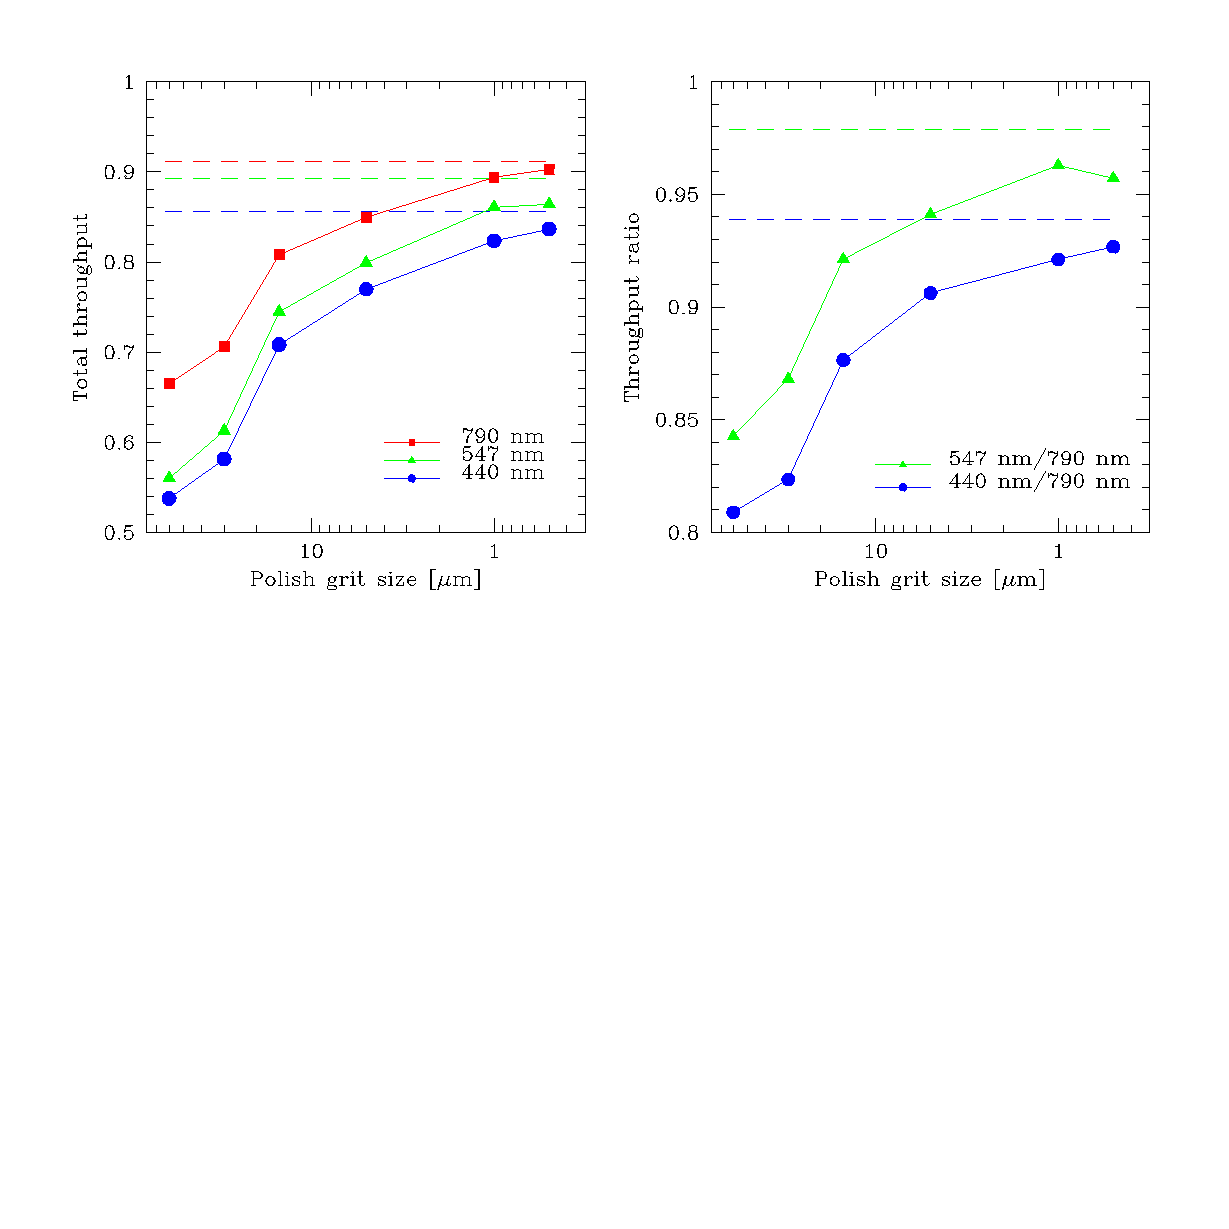
\includegraphics[width=\textwidth, trim=0 4in 0 0, clip=true]{FRD/figs/tput.eps}
  \caption[Total throughput as a function of wavelength and polish
    level]{\fixspacing\label{fig:tputwave} Total throughput as a function of
    polish grit for three different wavelengths (left), and the relative
    increase in \filtB and \filty referenced to \filtI (right). Dashed lines
    show the values expected from the product specifications. This is measured
    for a 17m length of FBP400440480 fiber.}
\end{figure}

\section{Angle Dependence}
\label{FRD:sec:angle}
\subsection{Experiment}
We are also interested in the dependence of FRD on the light input
angle. The direct beam injection method reported in
\S\ref{FRD:sec:direct} injects a full cone of light into a fiber,
i.e., the input beam contains rays incident on the fiber face from
normal up to half of the vertex angle of the cone.  To probe FRD
effects at single, discrete input angles (essentially an annular cone)
we use an experiment similar to the laser injection method of
\citet{Carrasco} and \citet{Haynes11}, but modified so that the far field fiber
output is imaged on to an opaque screen rather than through a
translucent screen. This was done to eliminate ring blurring that
occurs when imaging through a translucent object of finite thickness.

We also needed to ensure that the imaging screen was far enough away
from the output fiber face. The output images consist of a ring with a
radius corresponding to the laser input angle and a thickness that
varies depending on the amount of FRD present at that particular input
angle. We expect each ring to have an inherent width equal to the
diameter of the fiber, but this width is in a collimated beam while
any FRD scattering results in a slightly diverging beam. With this in
mind, the far field images were recorded at a far enough distance from
the fiber output face that the FRD smearing width described by
\citet{Carrasco} and \citet{Haynes11} (calculated to be $\sim
2.6^{\circ}$ for our fiber) dominated the ring width. At the distance
chosen the 300 \mum\ core of the fiber subtends $\sim 0.06^{\circ}$ on
the screen.  Unfortunately, our direct-imaging approach requires the
fiber output and camera to be off-axis (due to physical constraints),
resulting in elliptical ring images. Significant effort was expended
to model the geometric distortion caused by this method; our analysis
software does an excellent job of removing the distortion to produce
circular rings.

Data were taken at input angles of $\pm17^{\circ}$ ($\sim f$/1.6) in
increments of $0.5^{\circ}$. For simplicity we use the FWHM of the
ring profile as a first-order measure of for the amount of FRD,
ignoring here the intricacies of the profile shape
\citep{Haynes11,Carrasco}.

\subsection{Results}

\begin{figure}[ht]
\begin{center}
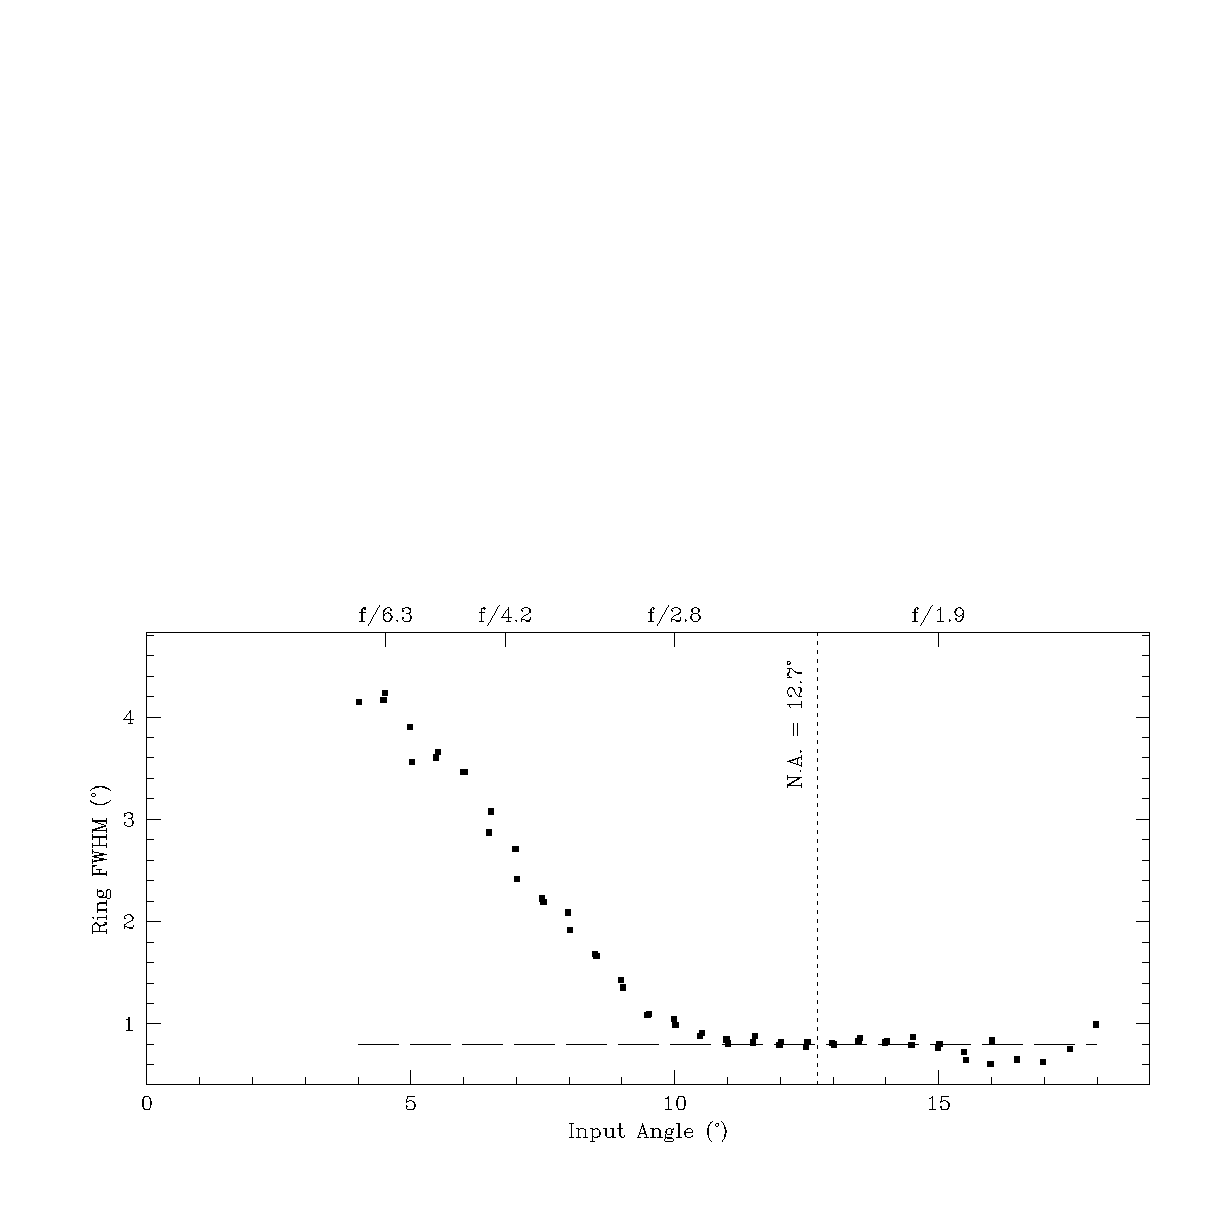
\includegraphics[width=\textwidth,trim=0 0.3in 0 3.8in,clip=true]{FRD/figs/angles.eps}
\caption[Dependence of FRD on input angle]{\fixspacing\label{fig:angle}
  Smearing due to FRD (ring width) as a function on input angle. The vertical
  dotted line marks the numerical aperture of the fiber specified by the
  vendor. The horizontal dashed line represents a best fit to the micro-bend
  model of \citet{Carrasco} over the full angular range
  of our data adopting $D=\val{1.15\times 10^{-6}}{m^{-1}}$. This value of $D$
  is constrained by a best-fit of the micro-bend model to our data in the
  range of 10 to 18 degrees.}
\end{center}
\end{figure}

Figure \ref{fig:angle} shows how the amount of ``smearing'' caused by
FRD (ring width) varies with different input beam angles. Angles below
$4^{\circ}$ are not plotted; future reports of this experiment will
measure ring widths in the regime where ring-width exceeds ring
radius.

The results in figure \ref{fig:angle} show that FRD effects are very
large at small angles, as expected, and decrease with increasing
angle until leveling out at $\sim 10^{\circ}$, which is within a few
degrees of the numerical aperture (12.7$^{\circ}$). It is possible to
extend the ring measurements to angles above the numerical
aperture. While the throughput decreases in this regime, the FRD
appears to remain fairly constant.

We have compared these trends to predictions of the micro-bend model
presented in \citet{Carrasco}.  We find a micro-bend parameter of
$D=\val{1.15\times 10^{-6}}{m^{-1}}$ provides the best fit to our data
(plotted in figure \ref{fig:angle}). This is a lower limit on the
value of $D$ for this fiber.  An upper limit on the value of $D$ comes
from matching the micro-bend model to our widest ring ($4^{\circ}$),
from which we find $D<\val{2.0\times 10^{-5}}{m^{-1}}$. For this range
of $D$, our measurements are in an angular regime where the micro-bend
model predicts a ring width nearly constant in angle. The fact that
our data show a non-constant ring-width indicates that this micro-bend
model is not a good description of the data and therefore not likely
the physical origin of FRD.

Our results are also important because they indicate just how strongly
FRD is dominated by light entering the fiber at smaller angles with
respect to the fiber optical axis. In astronomical applications,
fibers are typically fed by on-axis optical systems with central
obstructions from secondary and/or field-corrector optics. From an
entropy stand-point, i.e., information gathering-power per unit cost,
the central rays obscured are the least valuable. Consequently,
wide-field survey-telescopes \citep[e.g., SDSS, ][]{York00,Gunn06},
which are fast and have relatively large central obstructions, are
ideally suited to fiber coupling. Further analysis of data like that
in Figure 7 will allow us to quantify this statement.

\section{Summary}
\label{FRD:sec:summary}
Two experiments to 
measure the
amplitude of FRD as a function of wavelength, surface polish, 
and light-injection angle have been carried out and described.
The primary results are:
\begin{enumerate}

\item A component of FRD is attributable to the end-polish
  on fiber surfaces, however this appears to be a second-order effect
  relative to the impact of light-injection angle (beam speed) slower
  than \f3. FRD decreases with polishing down to finer grit sizes, but
  not significantly below grit-sizes of 5\mum.

\item Total throughput (light emerging at all angles) also depends on
  end-polish, with a wavelength dependence that indicates the increase
  in throughput is simply a reduction in surface-scattering.  The most
  significant gains occur for polishing that proceeds down to 5 $\mu$m
  grit, although for most astronomical applications at low
  light-levels polishing down to the finest grit is measurably
  advantageous.

\item The amount of FRD does \textbf{not} depend on wavelength, as found now
  in several experiments. This is in contrast to the predictions of micro-bend
  theory for FRD's origin \citep{Carrasco}.

\item FRD is dominated by light entering the fiber at smaller angles
  (in our case $<10^{\circ}$), as is well known. Measurements here
  allow us to quantify this statement in detail. The amplitude and
  angular dependence of FRD also do not agree with predictions from
  micro-bend theory.

\end{enumerate}

This work was supported by NSF grants ATI-0804576 and AST-1009471.

\bibliographystyle{thesis}
\bibliography{FRD}

\chapter[\GP Construction]{\GP and HexPak: A Variable-pitch, Dual-head IFU for the WIYN 3.5m Bench Spectrograph}
\label{chap:pak_build}
\epigraph{\fixspacing\emph{When the going gets weird, the weird turn
    pro}}{Raoul Duke}

% Leave space between title and quote or publication note.  This has often been
% 10cm for a quote and 8 cm for a reference, but this is really up to you.
%\vspace{8cm}

\vfill

\begin{flushright}
  \fixspacing
  \textit{A version of this chapter has previously appeared in\\
    \emph{Ground-based and Airborne Instrumentation for Astronomy IV. Proceedings of the SPIE}}\\
    \vspace{1ex}
    Wood, et. al. 2012. Volume 8446, article 84462W
\end{flushright}

%%%%%%%%%%%%%%%%%%%%%%%%%%%%%%%%%%%%%%%%%%%%%%%%%%%%%%%%%%%%% 
\begin{chabstract}
  We describe the design, construction, and expected performance of two new
  fiber integral field units (IFUs) --- HexPak and \GP --- for the WIYN 3.5m
  Telescope Nasmyth focus and Bench Spectrograph.  These are the first IFUs to
  provide formatted fiber integral field spectroscopy with simultaneous sampling
  of varying angular scales.  HexPak and \GP are in a single cable with a
  dual-head design, permitting easy switching between the two different IFU
  heads on the telescope without changing the spectrograph feed: the two heads
  feed a variable-width double-slit.  Each IFU head is comprised of a fixed
  arrangement of fibers with a range of fiber diameters.  The layout and
  diameters of the fibers within each array are scientifically-driven for
  observations of galaxies: HexPak is designed to observe face-on spiral or
  spheroidal galaxies while \GP is optimized for edge-on studies of galaxy
  disks.  HexPak is a hexagonal array of 2.9 arcsec fibers subtending a 40.9
  arcsec diameter, with a high-resolution circular core of 0.94 arcsec fibers
  subtending 6 arcsec diameter.  \GP is a 39 by 55 arcsec rectangular array
  with rows of fibers of increasing diameter from angular scales of 1.9 arcsec
  to 5.6 arcsec across the array.  The variable pitch of these IFU heads allows
  for adequate sampling of light profile gradients while maintaining the photon
  limit at different scales.
\end{chabstract}
\cleardoublepage

\section{INTRODUCTION}
\label{GPB:sec:intro}
HexPak and \GP are two new formatted fiber optic integral field units
(IFUs) for the WIYN 3.5m telescope Bench Spectrograph\footnotemark.
\footnotetext{The WIYN Observatory is a joint facility of the University of
  Wisconsin-Madison, Indiana University, Yale University, and the National
  Optical Astronomy Observatory.}  These two IFUs are unique because they are
the first formatted fiber IFUs to include multiple fiber diameters within the
same fiber head.  Including multiple fiber diameters allows each of these IFUs
to simultaneously sample different angular scales within the same observation.
The smaller fibers can gather light from higher surface brightness regions
(e.g.\ the core or midplane of a galaxy disk) while the larger fibers can
collect light from fainter, more diffuse regions (e.g.\ larger scale heights
or scale radii of a disk), thereby enabling high S/N measurements to be
obtained simultaneously at a range of spatial positions.


The two IFUs share the same cable and ``foot'' for mounting onto the WIYN
Bench Spectrograph.  Sharing the same cable minimizes the total volume
required for routing within the WIYN telescope in an already over-filled
system.  Sharing the same foot results in a unique dual-slit design, allowing
the two heads to be exchanged at the telescope without requiring changes to
the spectrograph system.  HexPak has a high-resolution core of fibers three
times smaller in diameter than the surrounding fibers.  As a hexagonal array
with a circular, high-resolution core, HexPak is tailored for studies of
radially-distributed, diffuse light sources, such as face-on galaxy disks,
spheroidal galaxies, or star clusters.  The \GP head consists of five
different fiber sizes, arranged in rows to form a gradient of fiber diameters
from one edge of the array to the other.  It is designed for integral field
spectroscopy of edge-on galaxies, making it well-suited for studying
extra-planar gas and stars in spiral galaxy disks.


Including multiple fiber diameters comes at a cost, however.  In the case
where the system spectral resolution is limited by the slit width, this will
result in a varying spectral resolution, inversely proportional to the fiber
diameter.  In this case the maximum resolution will change by a factor of 3
for \GP and 3.1 for HexPak, increasing from the largest to the smallest
fibers.  However, the smallest reimaged fiber sizes will have contributions
from optical aberrations from the spectrograph. As a result, we expect the
achievable resolution to increase only by a factor of 2--2.5 for HexPak.

The science impact of changing spectral resolution depends on the specific
application.  For example, the velocity dispersion of stars is expected to
increase with scale height above the disk midplane in edge-on disk galaxies.
For the study of stellar velocity dispersions in spheroidal or face-on disk
galaxies, as another example, it would be advantageous to \emph{increase}
spectral resolution with radius, since systems become dynamically colder
moving outward.  This is opposite what these instruments deliver.  On the
other hand, at lower surface brightness the limits of S/N prevent useful
information from being obtained at high spectral resolution, and in this sense
these instruments provide a practical balance between signal and resolution.
As we describe below, ample sky fibers are included for all fiber sizes to
ensure excellent sky subtraction.

This instrument follows in the legacy of the excellent WIYN fiber IFUs
DensePak \citep{Barden98} and SparsePak \citep{Bershady04,Bershady05}.  The
primary impetus behind this project was the increased throughput and image
quality of the newly redesigned WIYN Bench Spectrograph
\citep{Barden94,Bershady08,Knezek10}.  In the process an opportunity arose to
rebuild the decommissioned DensePak IFU.  The fiber from DensePak is being
reused for the larger fibers in the new HexPak array, and most of the hardware
in the cable ``foot'' housing that terminates the cable in the spectrograph
room at WIYN is reused from the DensePak cable.  HexPak contains additional
fibers that were newly purchased for this project.  \GP is made entirely using
new fiber.  Additionally, all the cabling and head mount hardware is newly
constructed.


In \S\ref{GPB:sec:design} we detail the key science drivers that served as a
design target for the instrument, as well as describe the design challenges
inherent in the design of formatted IFUs with multiple fiber diameters.  We
detail the construction process in \S\ref{GPB:sec:construction} and summarize the
project in \S\ref{GPB:sec:conclusion}.

%%%%%%%%%%%%%%%%%%%%%%%%%%%%%%%%%%%%%%%%%%%%%%%%%%%%%%%%%%%%%
\section{DESIGN} 
\label{GPB:sec:design}
%%%%%%%%%%%%%%%%%%%%%%%%%%%%%%%%%%%%%%%%%%%%%%%%%%%%%%%%%%%%%
\subsection{Science drivers} 
\label{GPBsub:sec:scidri}
These IFUs are designed for studying nearby galactic stellar populations, the
ISM of other galaxies, and stellar and gas kinematics of nearby galaxies.
Science drivers that influenced the design of the IFUs include: probing the
vertical structure of spiral disks using stellar and gas kinematic tracers;
studying the kinematics and abundances of diffuse ionized gas in edge-on and
face-on spiral galaxies; understanding the origin of winds in starburst
galaxies; measuring the rate of galactic outflows in normal spirals; and
connecting the properties of galaxy cores to the secular evolution of their
parent galaxies for E+A galaxies, QSO/AGN hosts, and pseudo-bulges.



%%%%%%%%%%%%%%%%%%%%%%%%%%%%%%%%%%%%%%%%%%%%%%%%%%%%%%%%%%%%%
\subsection{Head design} 
\label{GPBsub:sec:heads}
The primary limitations on the overall head size result from technical
limitations in the telescope and spectrograph system.  The maximum number of
fibers is limited simply by the maximum allowable slit length.  The overall
field of view is limited by the IFU mount on the telescope.  The IFU heads
mount into the WIYN Fiber-Optic Echelle (WIFOE) port on the telescope.  The
WIFOE port limits the overall head mount to a 1in circular diameter.
Accounting for mounting hardware, this limits the overall physical IFU head
size to approximately a square 0.5in$\times$0.5in, corresponding to a maximum
field of view (FOV) of $119\arcsec\times119\arcsec$ at the WIYN plate scale of
9.\farcs374/mm.  Packing fibers and head mount fixturing make the usable FOV
somewhat smaller than this, as shown later.


Each IFU head design presented a unique challenge for packing the fibers
together to form the heads.  The main problem we needed to overcome was one of
``circle packing'': what is the best way to arrange the fibers (represented as
circles as viewed along the optical axis of the system) so that we maximize
the focal plane filling factor in a compact region while achieving our target
scientific capability?  To our advantage, the problem of circle packing has
been relatively well-studied in the field of geometry.  For a single diameter,
the highest density packing arrangement is a hexagonal lattice arrangement as
used in both DensePak and the SparsePak array on WIYN, which results in a
packing density of $\pi/\sqrt{12} \approx 0.907$ \citep{Steinhaus99}.  Circle
packing becomes markedly more difficult when including more than one circle
diameter in the packing, as each of these new IFU heads does.  Our conceptual
goal for these IFUs was to enable the simultaneous sampling of varying surface
brightness levels in the same IFU observation.  To that end, the challenges of
circle packing were central to our ability to design these IFU heads in a way
that achieved our scientific goals yet were within our ability to fabricate.
In the following sections we describe the challenges we have overcome to
develop scientifically-useful head designs that were also feasible to
construct.


\subsubsection{HexPak}
\label{GPBsubsub:sec:hexhead}

\begin{figure}
    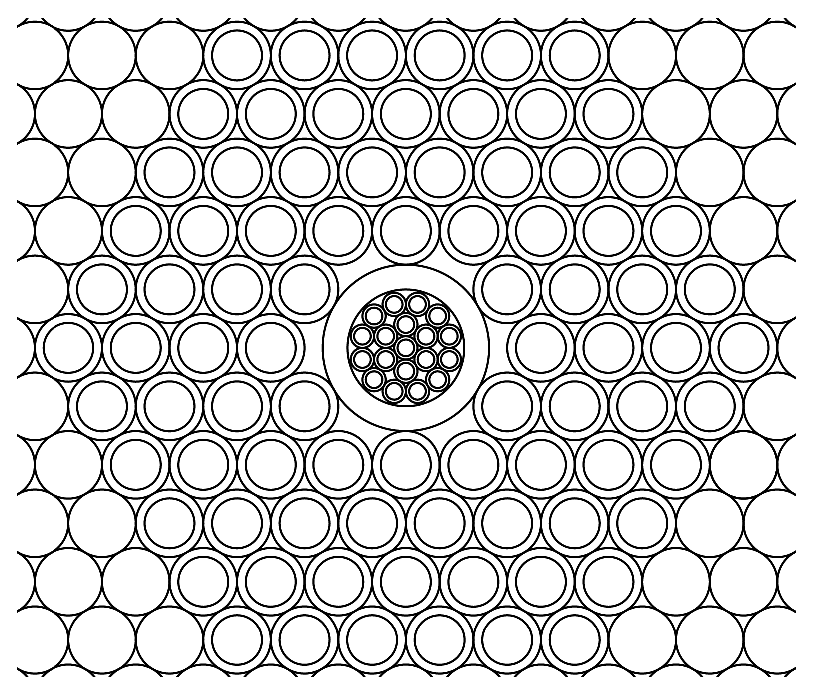
\includegraphics[width=0.48\textwidth]{Pak_build/figs/hexpak_zoom}
    \hfill
    \includegraphics[width=0.48\textwidth]{Pak_build/figs/19fibers}
    \vspace{1.5mm}
    \caption[HexPak Science Fibers]{\fixspacing \emph{Left:} Detail of the
      HexPak science fibers.  Fiber core regions are not shown for packing
      fibers.  The region depicted is approximately 0.18in$\times$0.15in
      centered on the hexagon.  \emph{Right:} Prototype of the HexPak core
      packing.  The fibers and capillary were glued into a 0.25in brass
      ferrule and ground to an even length in order to observe the quality of
      the packing.  This face has not been well-polished and does not
      represent our final target level of surface polish.
    \label{fig:hex_head}}
\end{figure}


The HexPak IFU head is designed to study objects with radial surface
brightness profiles (e.g.\ face-on galaxy disks, spheroidal galaxies).  As the
name suggests, HexPak is a hexagonal fiber array, based on a hexagonal lattice
arrangement.  As a result, the larger-diameter HexPak fibers are arranged in
the most compact manner possible.  The fiber diameter for the hexagonal region
was set by the diameter of the pre-existing DensePak fibers.  These fibers
have core diameters of 310$\mu$m and full outer diameters measured to be
$405\mu$m.  At the plate scale of the WIYN focal plane the cores of these
fibers span 2.\farcs8\ on the sky.  The design goal for the HexPak head was to
have a hexagonal region of fibers in an annulus around a high-spatial
resolution fiber core, necessitating two different fiber diameters.  There are
only nine possible compact\footnotemark\ packings of two circle diameters in a
plane \citep{Kennedy06}.  \footnotetext{A packing is ``compact'' if, for every
  circle \emph{C} that is tangent to a series of circles
  \emph{C}$_1$,\emph{C}$_2$,\dots,\emph{C}$_n$, circle \emph{C}$_i$ is tangent
  to circle \emph{C}$_{i+1}$ for $i = 1,2,\dots,n$.}  Of these, only one is
particularly relevant to the science goals of HexPak.  This packing involves
replacing one larger circle with an array of seven smaller circles (with a
diameter ratio of $\sim$0.386) while retaining the hexagonal lattice
arrangement of the other large circles (see Figure~1.e in
Ref.~\citenum{Kennedy06}).


The main flaw in this design as it pertains to our design goals is that the
seven smaller circles \emph{must} be surrounded by larger circles to maintain
a compact packing.  Stated differently, this arrangement dictates that the
high-resolution core of HexPak be no larger than the diameter of one large
fiber.  The reason behind this is that the largest radius occupied by the
seven smaller fibers is larger than the radius of the one fiber which was
removed.  Adjacent packings of seven small fibers would therefore overlap each
other.  This means that this packing arrangement would allow for higher
spatial sampling of no larger than a 2.\farcs8\ diameter region, but we felt a
larger region would more closely meet our science goals.  In order to achieve
a larger high-resolution core, we realized that this particular compact
packing can be reversed by instead replacing seven circles with one larger
circle.  This reversal ultimately led to the final design.


For the final HexPak head design we have replaced the central seven
2.\farcs8\ fibers in the hexagon with a glass capillary tube.  The outer
diameter of this tube is such that it packs compactly to the surrounding
fibers, and the inner diameter of the tube leaves a large, circular profile in
which we can pack small fibers.  Our final task was to determine how to
densely pack a moderate number of fibers inside this new circular aperture.
In order to determine an efficient packing within this aperture, we once again
turned to the study of circle packing.  A sub-field of circle packing
investigates the most efficient methods for packing circles of a given
diameter into one circle of a larger diameter.  Ref.~\citenum{Kravitz67}
presents empirically-derived optimal packings of circles into a circular
container.  For a diameter ratio of $\sim$0.206, it is possible to pack 19
small circles into one larger circle.  This final design of all the HexPak
object fibers can be seen on the left in Figure~\ref{fig:hex_head}.


It was prohibitively expensive to fabricate a form for a custom diameter
capillary draw just a few inches in length, so in practice our chosen diameter
(and the diameters of the fibers in the core) was limited to stock sizes.  In
the case of HexPak, our chosen glass capillary was purchased from Polymicro
Technologies\footnotemark\ and has a specified inner diameter of 750$\mu$m.
\footnotetext{Polymicro Technologies, 18019 N.\ 25th Avenue, Phoenix, AZ
  85023--1200, (602) 375--4100} This capillary inside diameter corresponds to
a core fiber outer diameter of about 154$\mu$m.  The closest stock fiber outer
diameter from Polymicro was 140$\mu$m (100$\mu$m or 0.\farcs94 core diameter),
resulting in the final design of 19 0.\farcs94\ fibers packed in the center of
the hexagon.  One sacrifice we make in using stock sizes is that there is a
2--3\arcsec\ gap between the core fibers and the larger fibers in the
hexagonal region.  The necessary outer diameter to fill the space of seven
405$\mu$m OD fibers is 1,050$\mu$m, but this capillary has an outer diameter
of 850$\mu$m.  This amount of undersizing is problematic for the packing
arrangement.  We manually thickened the pieces of capillary used in the head
by applying thin coatings of spray paint to the tubes until we reached the
desired diameter.


\begin{figure}[t]
    \centering
    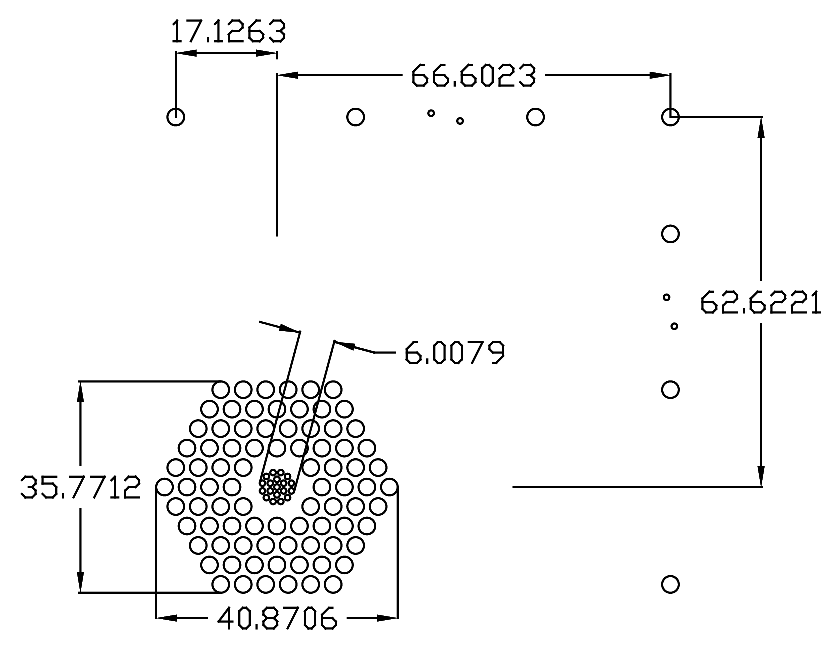
\includegraphics[width=.55\textwidth]{Pak_build/figs/hexpak}
    \hfill
    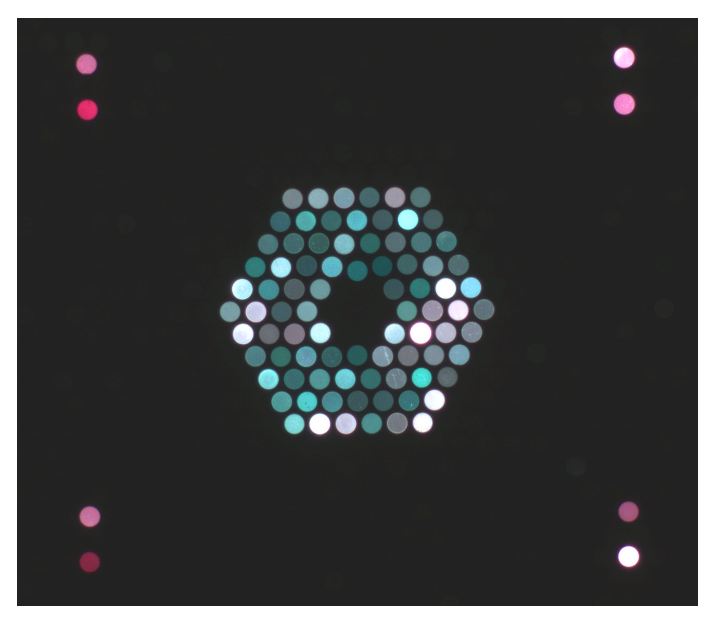
\includegraphics[width=.42\textwidth]{Pak_build/figs/hex_proto}
    \vspace{1.5mm}
    \caption[HexPak Design]{\fixspacing \emph{Left:} Head design for the
      HexPak IFU.  All displayed values are in units of arcseconds.  The two
      different fiber diameters are 2.\farcs8 and 0.\farcs94 on the sky.  Only
      the active fiber core regions are shown.  \emph{Right:} An image of an
      early prototype of the HexPak head design.  The center of the hexagonal
      region contains a hypodermic needle as a placeholder for the capillary
      with small fibers.  No small fibers are in the hypodermic shown here.
      The ends of the fibers were colored with marker to easily differentiate
      object fibers (green) from sky fibers (red).
    \label{fig:hexpak}}
\end{figure}


Although the results from Ref.~\citenum{Kravitz67} are empirical (and
therefore may not be compact) and our chosen fibers are slightly undersized,
the amount of extra space in the packing arrangement is at an appropriate
level to allow for mechanical tolerances.  We have successfully assembled two
prototypes of this packing and have high confidence that this will be viable
in the final head assembly.  The right side of
Figure~\ref{fig:hex_head} shows one of these prototypes after being
glued and roughly polished.


Our final head design is shown in Figure~\ref{fig:hexpak}.  The array design
has 114 total fibers.  Of these, the main science fiber region consists of 84
fibers with 2.\farcs8\ diameters contained within the outer hexagonal region
and 19 fibers with 0.\farcs94\ diameters spanning the central
6\arcsec\ diameter of the hexagon.  The capillary tube housing the
0.\farcs94\ fibers creates an annular gap 2--3\arcsec in radius between the
core fibers and the outer hexagonal region.  The array also has 11 total sky
fibers, seven with 2.\farcs8\ diameters and four with 0.\farcs94\ diameters.
The sky fibers are placed along the edges of the array opposite the science
fibers to maximize the separation between the object and sky sampling regions.
The sky fibers lie between 45\arcsec\ and 75\arcsec\ from the \emph{edge} of
the hexagon.  The HexPak head design employs nearly 1,000 short (3in) packing
fibers to fill the space in between the science fibers and the sky fibers,
similar to the scheme used for SparsePak.  The packing fibers also create a
roughly rectangular exterior head profile.  An early prototype of the HexPak
design is also shown in Figure~\ref{fig:hexpak}.  This prototype shows an
earlier revision in sky fiber arrangement and contains no small fibers in the
core of the array.


Ref.~\citenum{Bershady04} found that focal ratio
degradation\footnotemark\ (FRD) increases at the edge of the SparsePak array.
\footnotetext{Focal ratio degradation is a decrease in focal ratio of a beam
  as it passes through a fiber.}  They suggest several possible causes,
including stress incurred when releasing the head from its mold and pressure
introduced by the head-mount clamp.  Regardless of the cause, they recommend
leaving at least a 1.2mm buffer region at the outside of the head in order to
protect the active fibers from these potential stresses.  The ``packing
fiber'' buffer in the HexPak head is four large fibers, or about 1.6mm, which
we expect will alleviate FRD increases at the edge of the array.


\subsubsection{\GP}
\label{GPBsubsub:sec:gradhead}

\begin{figure}[t]
    \centering
    \begin{minipage}[c]{0.5\textwidth}
        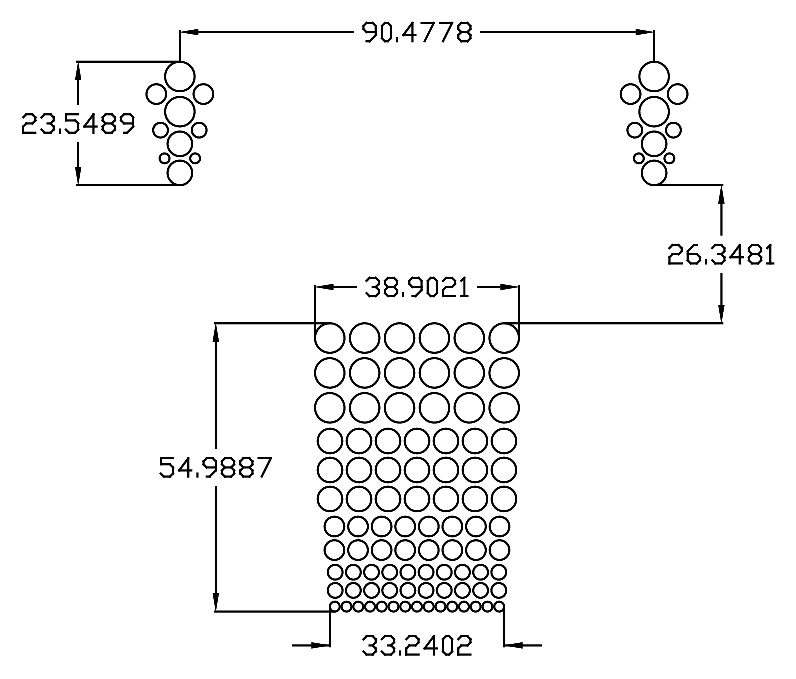
\includegraphics[width=0.95\textwidth]{Pak_build/figs/gradpak}
    \end{minipage}
    \hfill
    \begin{minipage}[c]{0.41\textwidth}
        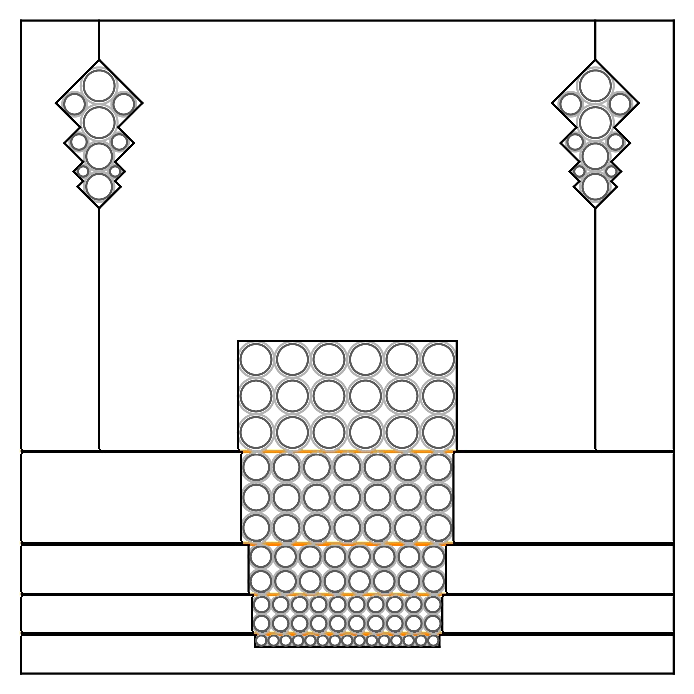
\includegraphics[width=0.95\textwidth]{Pak_build/figs/gradpak_zoom}
    \end{minipage}
    \vspace{1.5mm}
    \caption[\GP Layout]{\fixspacing \emph{Left:} Fiber layout for the \GP
      IFU.  All displayed values are in units of arcseconds.  The different
      fiber diameters are 1.\farcs9, 2.\farcs8, 3.\farcs7, 4.\farcs7, and
      5.\farcs6 on the sky.  Only the active fiber core regions are shown.
      \emph{Right:} Detail of the \GP head mount.  The darker gray circles
      are the active fiber cores, the lighter gray circles are the full
      O.D.\ of the fibers, and the orange lines represent $25\mu$m-thick
      plastic dividing layers.  The full exterior profile measures
      0.5in$\times$0.5in.
    \label{fig:gradpak}}
\end{figure}


\GP is designed to study objects that exhibit linear gradients in surface
brightness (e.g.\ edge-on galaxy disks, linear outflows).  Therefore, the
desired fiber arrangement in the head is linear rather than approximately
circular as it is in HexPak.  The design goal was to approximate layered
pseudo-slits of increasing slit width, accomplished by using stacked rows of
fiber, with fiber diameters increasing between rows.  There is no compact
packing of two different circle diameters that allows for each fiber size to
be arranged into linear, contiguous rows.  Circle packing theory did not show
obvious solutions for this problem, so we settled on a design that uses five
physically separated fiber regions, each containing only a single fiber
diameter.  This design is shown on the left in Figure~\ref{fig:gradpak}.  Our
final design includes a total of 110 fibers composed of five different fiber
core diameters: 200$\mu$m, 300$\mu$m, 400$\mu$m, 500$\mu$m, and 600$\mu$m.
Respectively, these fibers span angular diameters of 1.\farcs9, 2.\farcs8,
3.\farcs7, 4.\farcs7, and 5.\farcs6\ at the WIYN focal plane.  In order to
successfully accommodate five different fiber diameters within the same
packing arrangement, we have designed a layered head mount.


This head mount fixturing represents one of the largest engineering challenges
we have overcome.  In order to get each row of fibers to remain parallel to
each other, fibers of different diameters could not touch.  This is a result
of there being no compact packing of two different fiber diameters that allows
for parallel rows.  This meant that it would be impossible to use short
packing fibers in the \GP head.  After numerous iterations, we ultimately
designed a layered head mount that is assembled in stages, one fiber-diameter
region at a time.  The final head mount design can be seen on the right in
Figure~\ref{fig:gradpak}.  Each set of fibers of a given diameter is contained
by aluminum walls, precisely machined to the height of each fiber region.  The
head is then assembled by layering subsequent stacks of these segments on top
of one another.  All of the parts of the fixture are held together as an
assembly using small dowel pins that run the full height and width of the
assembly.  The main cavity was cut out as an assembly using a wire electric
discharge machining (EDM) process to ensure the best possible alignment
between adjacent fiber regions.  The \GP head block cavity was cut using a
0.004in diameter wire, allowing for a minimum corner radius of 0.002in
(50$\mu$m), small enough to ensure the smallest fibers fit into place.

The dimensions of the entire head block are 0.5in$\times$0.5in.  Each region
of fibers containing a single fiber diameter is separated from its neighbors
by a thin layer of plastic shim stock 0.001in (25.4$\mu$m) thick.  Although
this adds a gap between each region of fibers, the on-sky angular size of the
plastic layer is very small (0.\farcs24), which we deemed acceptable.  We have
successfully designed and assembled two prototype \GP head assemblies and
we are confident that this design is feasible.


The resulting array design consists of five stacked blocks of fibers arranged
into one or more rows, with the fiber core diameter increasing from 200$\mu$m
to 600$\mu$m between each block of fibers.  The entire block of science fibers
includes 90 fibers and covers an area on the sky roughly
35\arcsec$\times$55\arcsec.  The array also has two regions of sky fibers for
simultaneous sky measurements.  Each sky fiber region contains two fibers of
each fiber diameter included in the science fiber region.  The fibers in
\GP are arranged in a square lattice rather than in a hexagonal lattice,
reducing the effective filling factor within each fiber region.  This yields a
packing density of only $\pi/4 \approx 0.785$.  The advantage of this
arrangement is that the pseudo-slits within each region are vertically aligned
and are offset only in one dimension on the sky.


Since the entire \GP head mount assembly is composed of aluminum parts, no
short packing fibers are used in its design.  The design does, however, place
active fibers within 1.2mm of the edge of the head, inside the prescribed
minimum buffer distance.  However, we believe FRD edge effects should be
negligible due to the use of a stronger buffer material (aluminum in this
case) and the fact that at no point during assembly is any part of the \GP
head released from a mold.


%%%%%%%%%%%%%%%%%%%%%%%%%%%%%%%%%%%%%%%%%%%%%%%%%%%%%%%%%%%%%
\subsection{Slit design} 
\label{GPBsub:sec:slit}

\GP and HexPak both terminate in the same ``foot'' housing in a dual-slit
configuration.  The slit block uses a custom design that modified the
SparsePak slit block design.  The slit block assembly is made from two
separate aluminum plates, each specifically designed to create a pseudo-slit
for one of the IFUs.  Each pseudo-slit was created by cutting `v'-grooves into
the slit block.  The groove size, placement, and spacing is designed to match
the varying number and sizes of fibers in each IFU pseudo-slit.  A schematic
of the slit block assembly is shown in Figure~\ref{fig:slit}.  For mechanical
reasons, the fibers are aligned to be tangent to the optical centerline of the
slit, rather than being aligned by their centers.  The `v'-grooves were
precision-cut into the slit block using a wire EDM process like that used for
the \GP head mount fiber cavity, but with a smaller $0.002$in diameter
wire, resulting in a minimum corner radius of approximately $0.001$in
($25\mu$m).  This radius is smaller than the smallest fiber outer radius
(measured to be about 71$\mu$m) ensuring that even the smallest fibers will
sit nicely into the grooves.


We have set the fiber core edge-to-edge spacing at $291\mu$m to minimize
cross-talk while maximizing the number of fibers in the slit.
Ref.~\citenum{Bershady04} found that 400$\mu$m was the ideal edge-to-edge
spacing of fiber cores in the slit in terms of the trade-off between
cross-talk and packing density (i.e.\ total number of fibers).  However, this
determination was made using the old Bench Spectrograph system which was
upgraded in 2008 \citep{Bershady08}.  With improved image quality and detector
sampling as a result of the upgrade, we estimate we can reduce the fiber
spacing by $\sim25\%$ without introducing significant amounts of cross-talk
between fiber channels.


The fiber arrangements in the slit are informed by their locations within the
head design.  In HexPak, the hexagonal region is divided into six equal
wedges, each containing 14 fibers.  The fibers within each wedge are located
in the same region of the slit, with fibers near the core of the array being
located in the center of the slit segment.  Each wedge section in the slit is
separated from the adjacent wedge sections by a sky fiber, allowing sky
sampling across the entire slit length.  Three wedges and associated sky
fibers are located on each end of the slit, separated by all of the 0.\farcs94
fibers.  The 0.\farcs94 fibers are located in the center of the slit, with the
associated 0.\farcs94 sky fibers being located on either side of the
0.\farcs94 object fibers.  The \GP slit is sorted by fiber diameter.
Within each diameter region, each fiber row in the head is placed contiguously
in the slit, with sky fibers evenly distributed as separators between rows.


We also slightly modified the standard Bench Upgrade design for the ``toes''
of the cable in order to negate vignetting of the light exiting the fiber
slit.  The toes house the slit block and have open chambers for inserting
blocking filters, slit masks, and a back-illumination mirror.  These chambers
each have an aperture through which the exit beam must pass in order to reach
the spectrograph collimator.  We performed a vignetting analysis to determine
the maximum fiber slit width and slit length that could pass unvignetted
through the toes.  Ref.~\citenum{Bershady04} shows that, due to FRD, 99\% of
the energy in an \f6.3 input beam (the WIYN focal ratio) exiting the fibers is
contained within an \f4 output beam.  Therefore, as long as an \f4 beam could
pass through the toes without being blocked, we could consider light losses
from the toes to be negligible.  The SparsePak design for the toes allowed for
a maximum slit length of 79.8mm under this vignetting requirement.  This
number informed the fiber-to-fiber spacing for our final slit design,
resulting in an overall slit length of 76.6mm.  The maximum allowable slit
width for an \f4 beam was 1.23mm, or a $615\mu$m beam displacement from slit
center.  Our largest fiber has a $600\mu$m core diameter with approximately
$55\mu$m of clading and buffer in radius.  Each half of the slit block also
has a $25\mu$m plastic divider at slit center, a requirement of our slit block
construction process.  In total, the maximum beam displacement from slit
center is about $680\mu$m, too large for the standard design for the toes.  As
a result, we modified the design and increased the width of one critical
aperture in the toes such that the maximum allowable displacement from slit
center is $927\mu$m.


\begin{figure}[t]
    \centering
    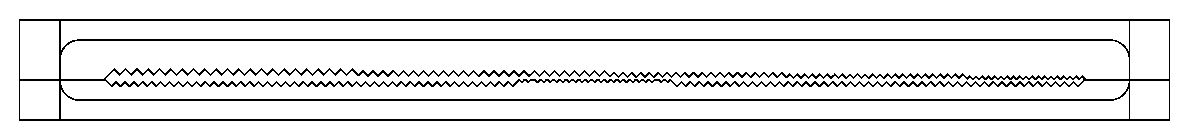
\includegraphics[width=\textwidth]{Pak_build/figs/slit}\\
    \vspace{2pt}
    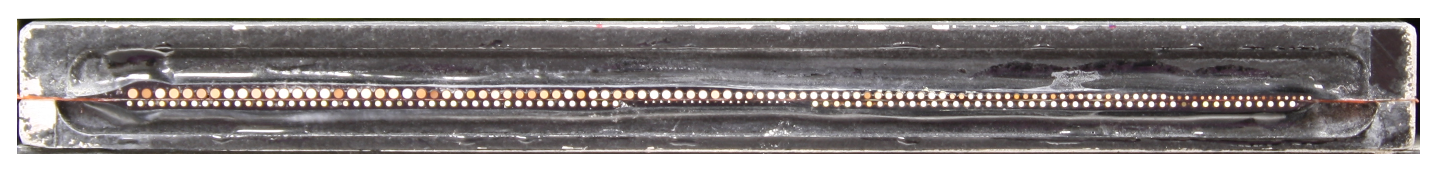
\includegraphics[width=\textwidth]{Pak_build/figs/slit_img}
    \caption[HexPak/\GP slit]{\fixspacing \emph{Top:} A schematic view of the
      slit block without fibers.  Both halves of the slit block assembly are
      shown.  The bottom set of grooves is the HexPak slit and the upper set
      of grooves is the \GP slit.  \emph{Bottom:} An image of the slit
      face in its current state.  The top row of fibers are \GP, arranged
      by decreasing diameters.  The bottom row of fibers are HexPak, with the
      0.\farcs94 fibers situated between the 2.\farcs8 fibers.  Brightness
      differences between fibers are largely due to surface irregularities in
      the unpolished head end.  Color differences are simply due to some
      fibers pointing at different parts of the lab.  The two 0.001in-thick
      plastic shim stock dividers are seen as a thin orange line separating
      the two slits.  The shown view spans 3.562in$\times$0.312in.
    \label{fig:slit}}
\end{figure}


%%%%%%%%%%%%%%%%%%%%%%%%%%%%%%%%%%%%%%%%%%%%%%%%%%%%%%%%%%%%%
\section{CONSTRUCTION AND STATUS} 
\label{GPB:sec:construction}

The design and construction of the SparsePak cable served as the starting
point for this instrument.  Technical details of SparsePak fabrication are
available in the Appendix section of Ref.~\citenum{Bershady04}.  In this
section we focus primarily on detailing the important features unique to this
instrument and noting significant departures from the SparsePak design.


At the present time, construction is complete on all cabling and the entire
spectrograph feed assembly (the foot).  Polishing of the fiber slit is nearly
complete, and final gluing and polishing of the IFU heads are scheduled to
conclude in June--August 2012.

\subsection{Fiber optics}
\label{GPBsub:sec:fibers}
The 91 2.\farcs8\ fibers that compose the hexagonal region and its associated
sky fibers are re-purposed from the DensePak IFU.  They have a specified
active core diameter of $310\mu$m and a measured total O.D.\ (including
cladding and buffer) of approximately $405\mu$m.  Ref.~\citenum{Barden98}
states that the DensePak fibers are similar to the Hydra FIP-type
``red-optimized'' fibers.  The 23 0.\farcs94\ fibers forming the
high-resolution core and associated sky fibers were purchased new from
Polymicro Technologies.  These new fibers are FBP-type broad-spectrum optical
fiber with excellent throughput for optical wavelengths.  The fibers have
silica cores with silica cladding and are designed to have excellent
throughput across the visible spectral window and into the near-infrared.  The
diameter specification (given as core:clad:buffer, in microns) is 100:120:140.
This new fiber is very similar to the fiber used in SparsePak and therefore we
expect similar throughput performance from the core HexPak fibers.

Throughput testing for SparsePak showed a roughly 20\% improvement in
throughput compared to the DensePak fibers, after accounting for differences
in fiber diameter and collected solid angle \citep{Bershady05}.  However, most
of the light loss in the DensePak cable was likely due to vignetting in the
original design of the fiber cable toes, before the Bench Upgrade.  With our
modified version of the standard Bench Upgrade toes, we expect these fibers to
have comparable performance to the SparsePak fibers in the red ($>4000$\AA;
the FBP-type fibers have better transmission properties below
4000\AA\ compared to the FIP-type fibers).

The \GP IFU consists entirely of new FBP-type broad-spectrum optical fiber
from Polymicro Technologies.  The fibers have specified diameters (given as
core:clad:buffer, in microns) of 200:220:240, 300:330:370, 400:440:480,
500:550:590, and 600:660:710.  This fiber is very similar to the fiber used in
SparsePak and therefore we expect similar throughput performance from all the
\GP fibers.


\subsection{Cabling}
\label{GPBsub:sec:cabling}
Each fiber is individually housed in a PTFE tube for protection and strain
relief.  The PTFE tubes for the $310\mu$m HexPak fibers were also re-used from
the DensePak cable.  All of the newly-purchased fiber is housed in new PTFE
tubing from Zeus, Inc\footnotemark.  \footnotetext{Zeus, Inc., 3737 Industrial
  Blvd., Orangeburg, SC 29118, (800) 526--3842} As a design decision to reduce
the radial cable size, the new PTFE tubes have ``light-weight wall''
thicknesses (0.006in in radius).  This has proven troublesome due to the
relative lack of radial strength and rigidity in the wall compared to
thicker-walled tubing.  The very thin walls of these tubes are prone to
kinking which threatens the integrity of the fibers they serve to protect.  We
recommend, at minimum, ``thin wall'' PTFE tubes ($\gtrsim$0.01in).


The PTFE tubes terminate at each end of the cable in metal shear clamps.  The
foot-end shear clamp contains an array of approximately $9\times27$ holes in a
three-element aluminum clamp.  The elongated design of this clamp serves to
transform the circular bundle of fibers into a rectangular shape approximating
the slit arrangement.  The head-end shear clamps are a similar three-element
design and function in a similar fashion to the foot shear clamp.  The hole
pattern in the head end shear clamps is roughly hexagonal in order to
accommodate the circular fiber bundle and to approximate the fiber layout of
the HexPak head.


The fibers and their PTFE tubes are encased in 75 feet of flexible metal
conduit.  The conduit housing the shared length of the cable consists of
approximately 57 feet of 2in ID IE30 and IE50\footnotemark\ interlocking
stainless steel exhaust hose.  \footnotetext{Penflex, Corp., 105B Industrial
  Drive, Gilbertsville, PA 19525, (800) 232--3539} This conduit retains
flexibility for handling while providing strength and durability for the
length of cable that will be enclosed within the telescope structure.


The remaining 18 feet of the cable is housed in two separate lengths of 1.25in
ID flexible aluminum standard electrical conduit.  Each length contains the
remaining length of fiber for one of the IFU heads.  The lightweight
construction and smaller diameter of this conduit allows for ease of handling
for mounting the IFU heads into the telescope's Nasmyth port.  These two
lengths of conduit are completely covered in polyolefin and PVC heat-shrink
tubing for additional rigidity and abrasion resistance.  The smaller lengths
of conduit are joined to the larger, stainless steel conduit through a
custom-built merge collector from the automotive industry\footnotemark.
\footnotetext{Specialty Design Products, Inc., 11252 Sunco Drive, Rancho
  Cordova, CA 95742, (888) 778--3312}


The conduit for each IFU head contains two custom-designed low-profile
rotation couplers.  Each coupler has $180^{\circ}$ of rotation about the
optical axis, allowing each IFU head to rotate a full $360^{\circ}$ with the
telescope instrument port rotator.  The two rotation couplers are spaced
approximately $12$in apart along the cable to ensure that the full rotation is
distributed along a sufficient length to avoid fiber stress.


\subsection{Fiber slit}
\label{GPBsub:sec:slitconstruct}
For gluing the fiber ends into the slit grooves, we fabricated custom metal
fixturing to bend the fibers 90$^{\circ}$ in the foot and hold them with
clearance to mount the slit blocks.  We used EPO-TEK\footnotemark\ 354
heat-curing optical epoxy to bond the fiber ends to the slit block.
\footnotetext{Epoxy Technology, Inc., 14 Fortune Drive, Billerica, MA 01821,
  (978) 667--3805} The gluing fixture held each fiber in its respective slit
position and allowed us to seat all the fibers simultaneously.  We used a thin
sheet of plastic to cover the exposed fiber and epoxy and held the fibers in
place using an aluminum pressing block while the epoxy cured.  We glued each
slit block separately and then constructed the final assembly from the two
completed halves.  The two halves are pinned together to ensure accurate,
repeatable positioning between the two slit halves.

\subsection{Fiber heads}
\label{subsec:headconstruct}
As tested with SparsePak and our HexPak and \GP test head assemblies, we
will use the same EPO-TEK 354 heat curing epoxy for assembling the IFU heads.
The HexPak head is assembled one row of fibers at a time, using short packing
fibers to fill in the spaces around the active fibers.  The 0.\farcs94\ fibers
are pre-assembled into their capillary tubes and then placed into the final
assembly during the gluing process.  For constructing the HexPak head, we
follow a design and process used for SparsePak, based on a concept from
S.\ Barden (\emph{private communication}).  We will assemble the fibers in a
micrometer-driven vice with the vice channel width set precisely to the width
of the head.  We will then use a precisely-machined tamping tool, just
slightly narrower than the width of the head, to pack the fibers into the
channel mold.  The mold and the tamping tool are sprayed with a PTFE mold
release\footnotemark[1]\ prior to gluing.  \footnotetext[1]{Miller--Stephenson
  Chemical Company, Inc., 55 Backus Ave., Danbury, CT 06810, (203) 743--4447}


The \GP head is assembled one fiber region at a time, with all fibers of a
single diameter being assembled at the same time.  The assembly is cured after
each additional region is assembled.  In contrast to the HexPak construction,
no vice is used for \GP.  The head mount parts are machined to the precise
cavity width to hold the fibers for each region, requiring only a pressing
plate to ensure the fibers remain seated in the cavity while curing.  The
pressing plate is coated in PTFE mold release as a precaution and separated
entirely from the epoxy by the plastic dividing layers, so at no point are the
fibers released from a cured mold.  This should alleviate any additional FRD
introduced through fiber stresses when releasing the mold, as seen in
SparsePak.


%%%%%%%%%%%%%%%%%%%%%%%%%%%%%%%%%%%%%%%%%%%%%%%%%%%%%%%%%%%%%
\subsection{Polishing}
\label{subsec:polishing}
We will polish the optical surfaces of the fiber slit and each of the fiber
heads in order to minimize light losses and FRD as the light passes through
the cable.  We are using an UltraPol\footnotemark[2]\ 1200 model lapping
machine with 8in diameter silicon carbide and aluminum oxide lapping disks.
\footnotetext[2]{ULTRA TEC Manufacturing, Inc., 1025 E.\ Chestnut Avenue,
  Santa Ana, CA 92701, (877) 542--0609} The lapping disks span a range of grit
sizes, starting from $70\mu$m for the grinding phase to $0.3\mu$m for the
final polishing phase.  Our laboratory testing shows that FRD is minimized for
surface roughnesses $<5\mu$m.  Our target surface roughness is $<0.5\mu$m.
See Eigenbrot et al.\ in these proceedings for a full description of our FRD
and surface polish testing.  At the time of this writing, the entirety of the
slit was polished at a 5$\mu$m level and ready to proceed to 1$\mu$m grit
disks, followed by 0.3$\mu$m grit.  An image of the slit in this state is
shown in Figure~\ref{fig:slit}.


%%%%%%%%%%%%%%%%%%%%%%%%%%%%%%%%%%%%%%%%%%%%%%%%%%%%%%%%%%%%%
\section{SUMMARY} 
\label{GPB:sec:conclusion}

We are in the final construction phase of two new fiber optic IFUs, \GP
and HexPak.  These IFUs will be the first formatted fiber IFUs to utilize
multiple fiber diameters within the same IFU head.  By including multiple
fiber diameters these IFUs will greatly expand the spectroscopic capabilities
of the WIYN 3.5m telescope, providing the ability to sample varying spatial
scales within the same observation with the highly versatile Bench
Spectrograph.  This will enable observations simultaneously spanning a wide
range in surface brightness to be optimized for the photon limit at spectral
resolutions between 1000 $< \lambda/\Delta\lambda <$ 30,000.


HexPak is designed to observe axi-symmetric surface brightness profiles with a
$36\arcsec\times41\arcsec$ hexagonal region sampled by 2.\farcs8\ fibers and a
6\arcsec diameter high-resolution core sampled by 0.\farcs94\ fibers.  \GP
is optimized for linear surface brightness gradients, with a stacked
pseudo-slit design spanning $39\arcsec\times55\arcsec$ using fibers ranging
from 1.\farcs9\ to 5.\farcs6\ in diameter.  Each of these IFUs presented
unique challenges for successfully incorporating multiple fiber diameters
within the same fiber head.  We have described two methods for overcoming
these challenges, one for radial arrangements of fibers and one for linear
arrangements.  Our solutions optimize the packing fraction of science fibers
while also achieving regular and precise placement and configuration of fibers
within each IFU.

\bibliographystyle{thesis}
\bibliography{Pak_build}

\chapter[Using \GP]{Observing NGC 891 with \GP: Novel Observational and Data Reduction Techniques}
\label{chap:gradpak_obs}

% Leave space between title and quote or publication note.  This has often been
% 10cm for a quote and 8 cm for a reference, but this is really up to you.
%\vspace{8cm}

%%%%%%%%%%%%%%%%%%%%%%%%%%%%%%%%%%%%%%%%%%%%%%%%%%%%%%%%%%%%% 
%% \begin{chabstract}
%%     Chapter abstract.
%% \end{chabstract}
%% \cleardoublepage

\section{Outline}
Using \GP presented its own unique set of challenges. In this chapter I will
detail the observation and reduction techniques I developed to get useful data
from this new IFU.

One question I have is where to put my GradPak\_guide. Much of the information
in that document will be reused in this chapter, but some of the lower-level
items (e.g. program API) seem out of place in a thesis. The whole guide will
live online somewhere and maybe the lower-level stuff can go in an appendix or
something, but I'm not so sure.

This chapter will also detail the observing program that resulted in our set
of NGC 891 data. Things like observing logs, pointings, etc. will go here. As
the end product of both the new reduction techniques and the NGC 891 program
we will show some reduced spectra and make some broad scientific
interpretations.

\section{Schedule}
Much of this writing is already done. More importantly, all of the
developement/analysis is complete. I estimate a week of focused effort is more
than enough to finish this chapter.

\bibliographystyle{thesis}
\bibliography{GradPak_obs}

\chapter[Stellar Populations in NGC 891]{The Location of Stellar Populations in NGC 891}
\label{chap:891_pop}

% Leave space between title and quote or publication note.  This has often been
% 10cm for a quote and 8 cm for a reference, but this is really up to you.
%\vspace{8cm}

%%%%%%%%%%%%%%%%%%%%%%%%%%%%%%%%%%%%%%%%%%%%%%%%%%%%%%%%%%%%% 
%% \begin{chabstract}
%%     Chapter abstract.
%% \end{chabstract}
%% \cleardoublepage

\section{Outline}
Kind of the ``meat'' of the thesis. Here we go in depth about the analysis
methods used on the data described in \ref{chap:gradpak_obs}. The punchline is
some statement about how age (and, to a lesser precision, metallicty) varies
with radius and height in NGC 891.

\section{Basic Analysis}
\begin{itemize}
  \item Velocities
  \item Emission Correction
  \item Extinction Model
\end{itemize}
\subsection{Schedule}
This is basically done. The two things that still need work are 1) deciding
where exactly the extinction model section goes, and 2) basic editing. This
could be completed in 2 days.

\section{LOS Depths}
\begin{itemize}
  \item Velocity-based measurement
  \item Optical depth based measurement
\end{itemize}
\subsection{Schedule}
Great progress has been made over the last few days on this front. I think the
velocity stuff is done and 80\% written up.

The optical-depth section of this has a completed framework, but the analysis
depends on a lot of assumptions about the dust distribution that we will take
from other sources. This requires more thought. Still, a week should be
sufficient to complete this section.

\section{SSP Fitting}
\begin{itemize}
  \item Basic model
  \item Chisq weights
  \item Model Libraries
  \item Determining Age/Metallicity
\end{itemize}
\subsection{Schedule}
The first three bullet points above are basically done and need only basic
copy editing. This could be done in a few days.

The last bullet point is where we have been spending most of our time recently
and I think we are extremely close to being ``done'' with the actual
analysis. I mean, shit, we could say ``we're going to use weights because they
exclude known bad metallicities, and we're going to use this power because
we've sampled a coarse grid of powers and it does the best in terms of
rejecting metallicities, but not too many metallicities'' tomorrow and be done
with this. The pipline to produce ages and metallicities already exists, we're
just iterating on the uncertainties.

Once the anlysis is done this will take a week to write up.

\section{Spectral Indices}
\begin{itemize}
  \item Measurement
  \item Use as independent check on metallicities used in SSP fitting
  \item Qualitative results of trends in age, metallicity with height
\end{itemize}
\subsection{Schedule}
Some of this is already done. The last bullet point needs the most work. In
particular I have not settled on exactly what plane of spectral indices are
the most informative. Trager and Co. like Balmer vs <MgFe> and Balmer vs <Fe>,
but the latter of those does not work well with our galaxy models (dynamic
range is very small). We currently use \Hd vs <MgFe> and \Hd vs Mgb, but the
justification is lacking.

I think if we stay relatively shallow on this topic we can get everything
figured out relatively quickly. Maybe 1-2 weeks.

\section{Heating Models}
\begin{itemize}
  \item Model recipe
  \item comparison to data
\end{itemize}
\subsection{Schedule}
The ball is mostly in your court on this one. We have ages as a function of r
and z, now we need models for comparison. In principle this could be a very
short, ``look, we're not crazy'' section with an eye towards future, in depth
work.

\bibliographystyle{thesis}
\bibliography{891_pop}

\chapter[Doppler Tomography]{Decoding 3D Disk Struction and Dynamics Using Doppler Tomography}
\label{chap:SALT}

% Leave space between title and quote or publication note.  This has often been
% 10cm for a quote and 8 cm for a reference, but this is really up to you.
%\vspace{8cm}

%%%%%%%%%%%%%%%%%%%%%%%%%%%%%%%%%%%%%%%%%%%%%%%%%%%%%%%%%%%%% 
%% \begin{chabstract}
%%     Chapter abstract.
%% \end{chabstract}
%% \cleardoublepage

\section{Outline}
Hey, remember all the fun with SALT data? I sure do. We got pretty damn close
to having something cool a few times. I think the most concise and impactful
realization of this analysis was the stuff I present at Galaxies in 3D across
the Universe in Vienna, 2014.

\section{Schedule}
This is pretty tricky. If we want to persue any new analysis the potential for
lots of work becomes very high. I estimate that even just pulling together all
the basic information from various posters/proceedings/paper drafts into a
coherent chapter will take a week.

\bibliographystyle{thesis}
\bibliography{SALT}

\chapter[Conclusion]{Conclusion}
\label{chap:conclusion}

% Leave space between title and quote or publication note.  This has often been
% 10cm for a quote and 8 cm for a reference, but this is really up to you.
%\vspace{8cm}

%\vfil\eject\clearpage
\clearpage
NGC 891 offers a unique opportunity to perform stellar poulation
analyis and compare the results to our detailed understanding of the
distribution of stars in the Milky Way. In this way it occupies an
important bridge between the Milky Way and surveys that offer a large
sample size, but a smaller spatial resolution. The closeness and
nearly totally edge-on nature of NGC 891 also allows for unambiguous
determination of finely sampled vertical gradients in stellar
population, which makes it a perfect test-case for theories concerning
the origin of disk stratification seen in the Milky Way.

To take advantage of the information available in NGC 891 I helped
design and construct HexPak/\GP, a pair of fiber IFUs for the WIYN
telescope. In Chapter \ref{chap:pak_build} I detail the design and
fabrication of these instruments. The important features of HexPak/\GP
are:
\begin{enumerate}
\item HexPak has a standard hexagon shape made mostly of fibers with
  an on-sky diameter of 2\farcs8. It also has a high resolution core
  of 18 0\farcs94 fibers that make it idealy suited for studies of
  face-on galaxies or any bright object where high spatial resolution
  is desired.

\item \GP is roughly rectangular in shape and has five different fiber
  sizes ranging from 1\farcs87 - 5\farcs62. The regions of different
  size are arranged in a gradient that is optimized for to measure
  roughly expoentially decreasing surface brightness at roughly
  \val{10}{Mpc}; a similar S/N per fiber can be achieved in a single
  exposure. \GP is ideally suited for observations of objects with a
  large dynamic range in brightness where spectral resolution can be
  sacrificed for observing efficiency.

\item At the spectrograph input the slits of HexPak and \GP share a
  foot and focal plane. This allows observers to swap between the two
  IFUs with zero modifications to the Bench Spectrograph.

\item The head fixtures of HexPak and \GP, while physically separate,
  share a common focal plane in the WIYN IAS. This further eases the
  transition between the two IFUs. In practice an observer can switch
  between HexPak and \GP during an observing run in roughly 10
  minutes.

\end{enumerate}

During the conception and construction of HexPak/\GP I researched ways
to improve the optical performance of fiber-based instruments, mainly
through the mitigation of FRD. In Chapter \ref{chap:FRD} I detail my
experiements, which are broadly applicable to all fiber optic systems,
and find:
\begin{enumerate}

\item FRD is dominated by light entering the fiber at smaller angles
  (i.e., closer to the axis of light propogation).

\item A secondary component of FRD is attributable to the end-polish
  of fiber surfaces. FRD decreases with polishing down to finer grit
  sizes, but not significantly below grit-sizes of 5\mum.

\item Total throughput also depends on end-polish, with a wavelength
  dependence that indicates the increase in throughput is simply a
  reduction in surface-scattering.  The most significant gains occur
  for polishing that proceeds down to 5 $\mu$m grit, although for most
  astronomical applications at low light-levels polishing finer than
  this level is measurably advantageous.

\item The amount of FRD does \textbf{not} depend on wavelength.

\end{enumerate}

Chapter \ref{chap:891_1} details the first set of results from a
program that measures stellar populations in NGC 891 with \GP. In this
chapter I detail challenges in data acquisition/reduction caused by
the unique nature of \GP, but also present methods that largely
eliminate any negative impact on the resulting data.

I also describe the observing program that is designed to cover NGC
891 out to large heights and radii. The design of \GP is ideally
suited to a program of this nature and allows for efficient collection
of high-quality data.

I then use the well known and characterized LICK spectral index system
to identify separate stellar populations in NGC 891 and find:
\begin{enumerate}

\item There is a clear transition with height above NGC 891's disk
  midplane between young and old populations at \val{0.4}{kpc}
  (roughly the broad-band exponential scale-height). This is
  consistent with models of heating of the stellar disk in the solar
  cylinder.

  \item For $|z| > \val{0.4}{kpc}$ there is a trend towards younger
    populations at larger projected radii, consistent with an
    inside-out formation history in NGC 891. The trend also suggests a
    flaring of the young stellar disk at radii beyond 8 kpc.

  \item Beyond 8 kpc in radius and between 0.4 kpc $\leq |z| <$ 1 kpc
    there is a a clear asymmetry in age between the two sides of the
    galaxy. The approaching side, where there is more H$\alpha$
    emission, appears younger. This can be explained by spiral
    structure in NGC 891; on the approaching side of the galaxy we see
    the leading edge of a spiral arm that has very recent/ongoing star
    formation. Our sight-lines to the receeding side of the galaxy,
    however, look onto the trailing edge of another arm that is
    obscured by high concentrations of dust.

\end{enumerate}

Finally, in Chapter \ref{chap:891_2} I employ the power of
full-spectrum fitting to get a detailed and quantitaive view of
stellar populations in NGC 891. To confidently interpret the results
of this method I need to understand the interplay between all of the
fit parameters, namely the well known degeneracies between age,
metallicity, and extinction. Furthermore, assumptions about the star
formation history in NGC 891 can introduce large systematics in our
results.

The degeneracies between age, metallicity, and extinction are
exacerbated by SSP template libraries that constitute a large set of
individual SSPs with little thought to the astrophysical similarities
that exist over a wide range of age and metallicity values. In other
words, most SSP template libraries have many SSPs that, while assigned
different age or metallicity values, have very similar spectra. To
mitigate these degeneracies I use diffusion k-means to create a new
SSP basis set that greatly reduces the number of SSP templates while
still preserving important astrophysical features. With this new SSP
basis set I estimate the uncertainty in fit parameters caused by
degeneracies between the model spectra to be roughly 10\% for age and
extinction and \asim 20\% for metallicity.

I also quantify the systematic age uncertainty that arises from
assuming a star formation history during the interpretation of the
fitting results. In the worst case these uncertainties are \asim 20\%,
but I argue that the worst case (totally random star formation on
small physical scales) is unrealistically pessimistic for our
data. NGC 891 is a coherent galaxy and over long timescales (\asim 1
Gyr) the star formation history should be relatively the same across
the entire galaxy. Thus the systematic uncertainties do not apply when
comparing detailed structure within NGC 891; they are only important
when comparing NGC 891 to other galaxies that may have different star
formation histories.

With an understanding of uncertainties in my results I identify three
features in NGC 891 that are distinct from one another in a position,
age, metallicity, extinction phase space. They are:
\begin{enumerate}

\item A ``primary'' disk that exists at all heights and radii less
  than \val{8}{kpc}. In this disk there is clear evidence for the
  presence of young stellar populations ($< \val{\asim 400}{Myr}$ ago)
  below \val{0.4}{kpc} and a lack of the same populations above
  \val{0.4}{kpc}, consistent with the results of Chapter
  \ref{chap:891_1}. Above this transition emission from the disk is
  dominated by intermediate and old stars and the average population
  age increases with height. This disk also exhibits negative
  metallicity gradients with both radius and height, which is
  consistent with observations of the Milky Way. It is also likely
  that the primary ``disk'' is actually a superposition of multiple
  disk components previously identified in NGC 891.

\item A flared extension of the the primary disk at radii beyond
  \val{8}{kpc}. This flare has the same age and metallicity properties
  as the main disk, but with a scale height roughly twice as
  large. This increase in scale height decreases the total surface
  density of dust at large radii and the extinction is correspondingly
  lower, especially near the midplane.
  
\item A sequence of intermediate-age, super-solar metallicity
  populations at large heights ($|z|> \val{\asim 0.9}{kpc}$) and radii
  ($r>\val{8}{kpc}$). Despite their old ages, the populations in this
  ``third sequence'' appear to come from a fundamentally different
  underlying distribution compared to stars at similar heights but
  smaller radii. Despite an overall higher metallicity this third
  sequence still shows internal metallicity gradients in $r$, and $z$
  consistent with the trends seen in the primary disk and flare. The
  origin of this population is not easily explained and any theories
  about it will need to contend with its curious combination of old
  ages and high metallicities that occur far from the center of the
  galaxy.

\end{enumerate}

This work constitutes one of the first detailed, resolved studies of
stellar populations in a nearby galaxy and as such lays the groundwork
for future studies. In particular, the methods outlined here could
easily be applied to other nearby, edge-on galaxies. This thesis
provides a robust set of tools, from instruments to data reduction and
analysis methods, that will allow future astronomers to rapidly expand
our view of stellar populations and disk formation.

\clearpage
\phantomsection % Fixes references link in hyperref/PDF index

% Requires thesis.bst to be present (or linked) in chapter subdirectory.
\bibliographystyle{thesis}
\bibliography{Introduction}


% See the thesis.cls file for the steps to convert AASTeX papers
% into thesis chapters

%%%%% ADD APPENDICES %%%%%%%%%%%%%%%%%%%%%%%%%%%%%%%%%%%%%%%%%%%%%%%%%%%%%%%%%%%

%\addtocontents{toc}{\protect\vspace{0.5cm}}
                        % Add some vertical space to the table of contents
                        %   file before listing the appendices (the \protect
                        %   command is necessary because \vspace is fragile).

%\appendix		% Resets chapter numbering to A, B, C... for appendices

%\include{apA}		% *.tex file for Appendix A (just like a chapter)

%\include{vitae}         % *.tex file for the Vitae

%\include{colophon}      % *.tex file for the Colophon

% END THE DOCUMENT %%%%%%%%%%%%%%%%%%%%%%%%%%%%%%%%%%%%%%%%%%%%%%%%%%%%%%%%%%%%%

%\clearpage
%Need to uncomment all of the following to get an index
%\addcontentsline{toc}{section}{Index}
%{\fixspacing \small
%\printindex
%}

\end{document}
